\documentclass[11pt]{article}
\usepackage{geometry}                % See geometry.pdf to learn the layout options. There are lots.
\geometry{letterpaper}                   % ... or a4paper or a5paper or ... 
%\geometry{landscape}                % Activate for for rotated page geometry
%\usepackage[parfill]{parskip}    % Activate to begin paragraphs with an empty line rather than an indent
\usepackage{booktabs} % for much better looking tables
\usepackage{array} % for better arrays (eg matrices) in maths
\usepackage{paralist} % very flexible & customisable lists (eg. enumerate/itemize, etc.)
\usepackage{amssymb, amsmath}
\usepackage{epstopdf}
\usepackage{amsthm}
\usepackage{amsfonts}
\usepackage{graphicx}
\usepackage{amsmath}
\usepackage{mathtools}
\usepackage{amssymb}	
\usepackage{float}
\usepackage{leqno}
\usepackage{wrapfig}
\usepackage{mathrsfs}
\usepackage{nomencl}
\usepackage{fancyheadings}
\usepackage{fancyhdr}
\usepackage{import}
\usepackage{tfrupee}
\usepackage{hyperref}
\usepackage[]{algorithm2e}
\usepackage{bbm}
\usepackage{courier}
\usepackage{wasysym}
\usepackage{tikz}
\usetikzlibrary{bayesnet}
%\usepackage{mcode}
\newtheorem{mydef}{Definition}[section]
\newtheorem{myprop}{Proposition}[section]
\newtheorem{mytheorem}{Theorem}[section]
% numbers on equations
%\numberwithin{equation}{section}

%\DeclareGraphicsRule{.tif}{png}{.png}{`convert #1 `dirname #1`/`basename #1 .tif`.png}
%\maketitle
\title{Coal mine disasters - constructing a complex MCMC algorithm}
\author{Eric Leijonmarck 870820-0095 \and Victor Tingstr\"{o}m 910101-0651}
\date{19 March, 2014}


\begin{document}
\begin{titlepage}

\begin{center}


\includegraphics[scale=2]{kth}
\\[\baselineskip]
{\LARGE 
SF2955, Home Assignment 2, Complex MCMC}

\end{center}

\begin{minipage}{0.5\textwidth}\begin{flushleft}
\emph{Authors:}
\end{flushleft}\end{minipage}
\begin{minipage}{0.5\textwidth}\begin{flushleft} 
\end{flushleft}\end{minipage}\\
\begin{minipage}{0.5\textwidth}\begin{flushleft} 
Eric \textsc{Leijonmarck}\\
870820-0095\\
\end{flushleft}\end{minipage}
\begin{minipage}{0.5\textwidth}\begin{flushright} 
\textit{ericle@kth.se}\\
\end{flushright}\end{minipage}\\\\
\begin{minipage}{0.5\textwidth}\begin{flushleft} 
\end{flushleft}\end{minipage}\\
\begin{minipage}{0.5\textwidth}\begin{flushleft} 
Victor \textsc{Tingstr\"om}\\
911109-0651\\
\end{flushleft}\end{minipage}
\begin{minipage}{0.5\textwidth}\begin{flushright} 
\textit{vtin@kth.se}\\
\end{flushright}\end{minipage}\\\\
\begin{minipage}{0.5\textwidth}\begin{flushleft} 
\emph{Supervisor:}\\
\end{flushleft}\end{minipage}
\begin{minipage}{0.5\textwidth}\begin{flushleft} 
\end{flushleft}\end{minipage}\\
\begin{minipage}{0.5\textwidth}\begin{flushleft} 
Jimmy \textsc{Olsson}
\end{flushleft}\end{minipage}
\begin{minipage}{0.5\textwidth}\begin{flushright} 
\textit{jimmyol@kth.se}
\end{flushright}\end{minipage}
\vfill
\begin{center}
{\large \today}
\end{center}
%Date of submission: September 28, 2012
\end{titlepage}

\section*{Coal mine disasters - Constructing a complex MCMC algorithm}

\subsection*{Introduction}

For this exercise, we analyze a time series containing the British coal mining disasters under the time period 1851--1962. The difference between this exercise and the one in the course literature, is that we have a continuous time series as well as more than 1 \textbf{breakpoint}. A breakpoint is thus the year at which the intensity of the disasters change. We will use $d-1$ breakpoints, where $d$ then corresponds to the number of intervals we will use. In order to get a feel for the time series we will analyze, a figure containing a histogram of the disasters is found in figure \ref{fig:disasters}.

\begin{figure}[H]
  \centering
    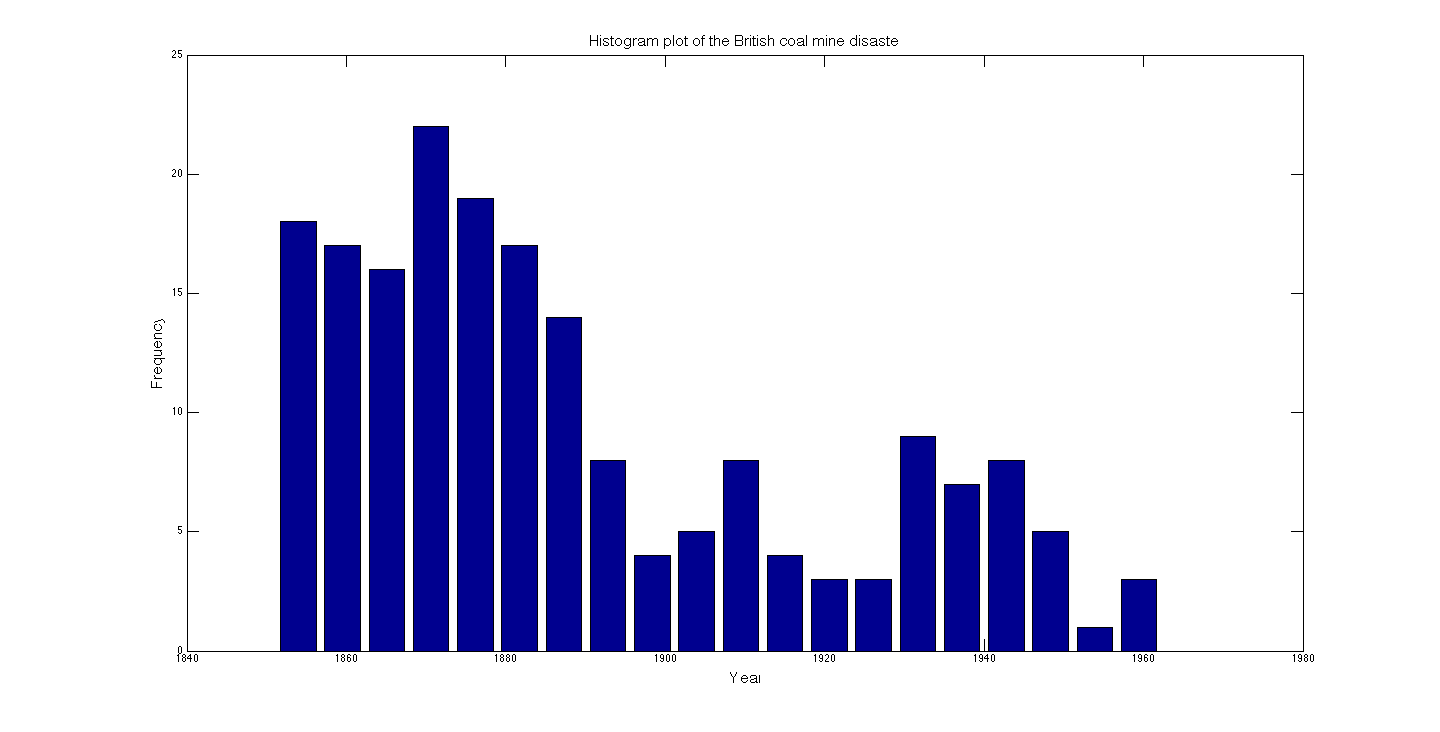
\includegraphics[scale=0.24]{./Figures/disasters.png}
  \caption[An Electron]{Histogram plot of the British coal mine disasters in the time period 1851--1962.}
  \label{fig:disasters}
\end{figure}

As is seen in figure \ref{fig:disasters} there is a change in the disaster intensity at the turn of the century, perhaps due to some legislation regarding work safety or some technological advancement. \\ \\ To begin the exercise, we define the vector $\boldsymbol{t}$ to be the vector containing all of the breakpoints $t_i, \: i = 2,\dots d$ aswell as the start and end point $t_1 = 1851$ and $t_{d+1}=1963$. We wish to model the disasters using an inhomogenous Poisson process with an intensity $\lambda_i$ for each of the intervals $[t_i,t_{i+1}), \: i = 1,\dots,d$. Where all of the $\lambda_i$'s are collected in a vector $\boldsymbol{\lambda}$. \\ We will denote the time series containing the year at which disaster struck as $\boldsymbol{\tau} = (\tau_1,\dots,\tau_n)$ for $n = 191$, where the subscript denotes accident $i$. \\ We then define the number of accidents under the interval $[t_i,t_{i+1})$ to be
\[n_i(\boldsymbol{\tau}) = \sum^n_{j = 1}\mathbbm{1}\{[t_i,t_{i+1})\}\cdot \tau_j \]
We set a $\Gamma(2,\theta)$ prior on the intensities, $\lambda_i$, and a $\Gamma(2,\beta)$ hyperprior on $\theta$. Where $\beta$ is a hyperparameter that needs to be specified. Furthermore, we put the prior
\[ f(\boldsymbol{t}) \propto\left\{
	\begin{array}{l}
		\prod^d_{i = 1}(t_{i+1} - t_i), \quad \text{for } t_1 < t_2 < \dots < t_{d+1} \\
		0, \quad \text{else} 
	\end{array}
\right. \]
 This prior prevents the breakpoints from being located to closely. All of these prior assumptions then imply that 
\[f(\boldsymbol{\tau} | \boldsymbol{\lambda}, \boldsymbol{t}) \propto \prod^d_{i = 1}\lambda_i^{n_i(\boldsymbol{\tau})}\cdot\exp \left \{ - \sum^d_{i = 1}\lambda_i(t_{i+1} - t_i) \right \} \]
In order to sample from the posterior $f(\theta,\boldsymbol{t},\boldsymbol{\lambda} | \boldsymbol{\tau})$ we will construct a hybrid \textbf{M}arkov \textbf{C}hain \textbf{M}onte \textbf{C}arlo algorithm, where the hybrid comes from the fact that we will need to sample $\boldsymbol{t}$ using a Metropolis--Hastings step whereas the other components can be updated using a Gibbs sampler. \\ \\ There are several ways to choose the proposal distribution for the Metropolis--Hastings, we chose to use the \textit{Random walk proposal}, which means that we will update one breakpoint at a time and for each breakpoint $t_i$ generate a candidate $t^*_i$ according to
\[t^*_i = t_i + \epsilon, \quad \epsilon \sim \text{Unif}(-R,R) \]
Where $R = \rho(t_{i+1} - t_{i-1})$ and $\rho$ is a tuning parameter.

%Basic idea of MCMC (Markov Chain Monte Carlo): To sample from a density f we construct a
%Markov chain having f as stationary distribution. A law of
%large numbers for Markov chains guarantees convergence. \\

%MCMC is widely used for sampling, due to its simplicity when dealing with complex distributions or distributions of high dimensions. However, the price is that the samples will be statistically dependant. It can be used to simulate a probabiltiy distribution $\pi(x)$ that is known only up to a normalizing constant, which is especially important in Bayesian inference with $\pi$ as the posterior distribution.


\subsection*{a)}

For this exercise, we are supposed to find the marginal posteriors for $f(\theta| \boldsymbol{\tau}, \boldsymbol{t}, \boldsymbol{\lambda})$, $f(\boldsymbol{\lambda}|\theta,\boldsymbol{t},\boldsymbol{\tau})$ and $f(\boldsymbol{t}|\theta, \boldsymbol{\lambda},\boldsymbol{\tau})$. We began this exercise by identifying the different dependences , which are found in the following figure. 
  \begin{center}
      \tikz{ %
        \node[latent] (tau) {$\tau$} ; %
        \node[latent, left=of tau, yshift=0.5cm] (lambda) {$\lambda$} ; %
        \node[latent, left=of tau, yshift=-0.5cm] (t) {$t$} ; %
	\node[latent, left=of lambda, yshift = 0cm](theta){$\theta$};
	\node[latent, left=of theta, yshift = 0cm](beta){$\beta$};
	\edge{beta}{theta}
        \edge{theta}{lambda}
	\edge {lambda,t} {tau} ; %
      }
  \end{center}
Now that we've identified all of the dependences, we begin by analyzing the first posterior.
\begin{itemize}
\item[I.] We begin by rewriting the expression using \textit{Bayes' Theorem}
\[f(\theta| \boldsymbol{\tau}, \boldsymbol{t}, \boldsymbol{\lambda}) \propto f(\theta) \cdot f(\boldsymbol{\tau}, \boldsymbol{t}, \boldsymbol{\lambda}|\theta) \]
The second term is rewritten as
\[f(\boldsymbol{\tau}, \boldsymbol{t}, \boldsymbol{\lambda}|\theta) = f(\boldsymbol{\tau}|\boldsymbol{\lambda},\boldsymbol{t},\theta) \cdot f(\boldsymbol{t},\boldsymbol{\lambda}|\theta) \]
We then notice that there's independence between some of the variables, which then means that the expression is rewritten into
\[ f(\boldsymbol{\tau}|\boldsymbol{\lambda},\boldsymbol{t})\cdot f(\boldsymbol{t}) \cdot f(\boldsymbol{\lambda}|\theta) \propto f(\boldsymbol{\tau}|\boldsymbol{\lambda},\boldsymbol{t}) \cdot f(\boldsymbol{\lambda}|\theta) \]
Inserting this expression then yields
\[ f(\theta| \boldsymbol{\tau}, \boldsymbol{t}, \boldsymbol{\lambda}) \propto f(\theta) \cdot  f(\boldsymbol{\lambda}|\theta)  \cdot f(\boldsymbol{\tau}|\boldsymbol{\lambda},\boldsymbol{t})\]
The explicit expression for the distribution then becomes
\[ f(\theta | \boldsymbol{\lambda},\boldsymbol{t},\boldsymbol{\tau}) \propto \theta \cdot \exp\{-\beta\cdot\theta\}\cdot \theta^{2d}\prod^d_{i = 1}\lambda_i\cdot \exp \left \{ -\theta \sum^d_{i=1}\lambda_i \right \}\prod^d_{i=1}\lambda_i^{n_i(\boldsymbol{\tau})}\cdot \exp \left \{ - \sum^d_{i = 1}\lambda_i(t_{i+1} - t_i) \right \} \]
We then identify the terms containing $\theta$ and finally get that
\[f(\theta | \boldsymbol{\lambda},\boldsymbol{t},\boldsymbol{\tau}) \propto \theta^{2d + 1}\exp\left \{ -\theta \cdot \left ( \beta + \sum^d_{i = 1}\lambda_i \right) \right \} \sim \Gamma\left (2(d + 1), \beta + \sum^d_{i = 1}\lambda_i\right )\]
\item[II.] For economy of text, the entire proof of the distribution will be left out, the procedure is the same as in I. 
\[f(\boldsymbol{\lambda} | \boldsymbol{\tau},\boldsymbol{t}, \theta) \propto f(\boldsymbol{\tau} | \boldsymbol{t}, \boldsymbol{\lambda}) \cdot f(\boldsymbol{\lambda}|\theta) \cdot f(\theta) \]
Whose explicit expression is
\[f(\boldsymbol{\lambda} | \boldsymbol{\tau},\boldsymbol{t}, \theta) \propto \prod^d_{i=1}\lambda_i^{1 + n_i(\boldsymbol{\tau})}\cdot \exp\left \{ - \sum^d_{i = 1}(\theta + (t_{i+1} - t_i))\lambda_i \right \}  \]
Which implies that 
\[ \lambda_i \sim\Gamma \left ( 2 + n_i(\boldsymbol{\tau}), \theta + (t_{i+1} - t_i) \right ) \]
\item[III.] We are now supposed to calculate the posterior for 
\[f(\boldsymbol{t} | \boldsymbol{\tau},\boldsymbol{\lambda},\theta) \]
If one proceeds as in the previous examples, we will see that we cannot determine the distribution of $\boldsymbol{t}$ explicitly. This then means that we need to use the Metropolis--Hastings algorithm in order to sample $\boldsymbol{t}$. If one proceeds as in the previous examples, we will get that 
\[f(\boldsymbol{t} | \boldsymbol{\tau},\boldsymbol{\lambda},\theta) \propto \prod^d_{i = 1}(t_{i+1} - t_i)\lambda^{n_i(\boldsymbol{\tau})}\cdot\exp \left \{ -\sum^d_{i = 1}\lambda_i(t_{i+1} - t_i) \right \} \sim \frownie\]
\end{itemize}



\subsection*{b)}

Here we construct our hybrid MCMC algorithm to sample from the posterior $f(\theta,\boldsymbol{\lambda},\boldsymbol{t}|\boldsymbol{\tau})$. All components except the breakpoints $\boldsymbol{t}$ have been updated using Gibbs sampling, which is explained in further down in this section. The Metropolis--Hastings algorithm is explained below and has been used for the posterior of $\boldsymbol{t}$. Where we, as already mentioned, used a symmetric proposal for the proposal kernel. We will now briefly discuss the two different algorithms used for sampling.
\begin{itemize}
\item{The \textbf{Metropolis--Hastings} algorithm is an algorithm that is used for sampling from high--dimensional and/or complicated distributions that are for example only known up to a normalizing constant. The idea behind the MH algorithm is to choose a transition density $q$ almost arbitrarily. However, this density will not give the desired asymptotic distribution $f$, i.e. the distribution from which you wish to sample. We correct this by introducing a new transition density $\hat{q}$ using $q$ and a probability $\alpha(x,x^*)$ where $x$ is the current level and $x^*$ is a proposal. The proposal $x^*$ is rejected with probability $1 - \alpha(x,x^*)$. In order for the global balance equation to be satisfied, we must have that $\alpha(\cdot,\cdot)$ is defined as 
\[\alpha(x,x^*) = \min \left ( 1, \frac{f(x^*)q(x|x^*)}{f(x)q(x^*|x )} \right ) .\]
Since we now have a quotient, we can easily sample from distributions known only up to normalizing constants.
In our case we have, as already mentioned, a symmetric proposal. Which practically means that $q(x^*|x ) = q(x|x^* )$ and the two right terms of the quotient cancel out. The MH algorithm is explained briefly in figure \ref{fig:metrohast}.
\begin{figure}[H]
  \centering
    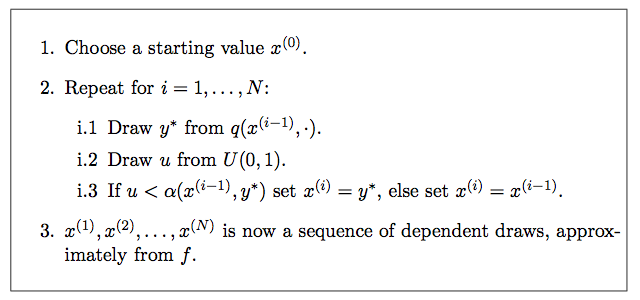
\includegraphics[scale=0.34]{./Figures/metrohast.png}
  \caption[An Electron]{Overview of how the Metropolis--Hastings algorithm works. The figure is taken from the lecture notes by Martin Sk\"old.}
  \label{fig:metrohast}
\end{figure}
}

\item{The \textbf{Gibbs sampler} algorithm is a Markov Chain Monte Carlo (MCMC) algorithm for obtaining a sequence of observations, which in turn can be approximated from a multivariate probability distribution. Typically the Gibbs sampler is used to approximate joint distributions, marginal distributions of one variable or computing an integral, when some of the variables are known observations, and is not in need of sampling. As this a MCMC algorithm, Gibbs sampling generates a Markov Chain of samples, hence the beginning of the chain may not accurately describe the desired distribution and one may want to remove the burn-in of the chain. Below a brief description of the algorithm is presented

\begin{enumerate}
	\item{Assuming we want to sample from multivariate distribution f on X. Assuming that X can be divided into blocks.}
	\item{We denote $x^k$ by the \textit{k}th component and $x^{-k}$ by the remaining components. Assuming that it is easy to simulate from $f_k(x^k|x^{-k}),\forall k$, i.e. the conditional distribution of $X^k$ given the other components.}
	\item{Now, simulating a sequence $X_k$, forming a Markov Chain on X, with the following properties: Given $X_k$, draw $X_{k+1}^n \sim f_n(x^n|x^{-n})$.}
\end{enumerate}
}
\end{itemize}


%\textit{Random walk proposal:} update one breakpoint at a time. For each breakpoint $t_i$ we generate a candidate $t_i^*$ according to

%\begin{equation*}
%t_i^*=t_i+\epsilon, \quad \text{with} \quad \epsilon \sim U(-R,R), \quad R=\rho(t_{i+1}-t_{i-1}
%\end{equation*}
The symmetric proposal yields a correct MCMC algorithm, as long as the proposal kernel specifies an irreducible aperiodic Markov Chain. The algorithm will generate a reversible Markov Chain with stationary distribution $\pi$, assuming that $\chi$ is a subset of $\mathbb{R}^k$ and the transition kernel $r(z|x)$ and $\pi(z)$ are densities on $\chi$. \\

The proposed kernel yields a correct MCMC as we have introduced a symmetric proposal, thus
\begin{equation}
r(z|x)=r(x|z), \quad \forall (x,z) \in t
\end{equation}
%http://dept.stat.lsa.umich.edu/~yvesa/afmp.pdf
implying that we can reach each state from any state and is non-periodic, i.e. an irreducible aperiodic Markov Chain.


\newpage
\subsection*{c)}
To start the exercise, we consider the amount of necessary samples used as burn-in, which we set to $N = 100,000$ samples. The following figure shows the draws of $\boldsymbol{t}$ for $d=2$, i.e. one breakpoint.

\begin{figure}[H]
\centering
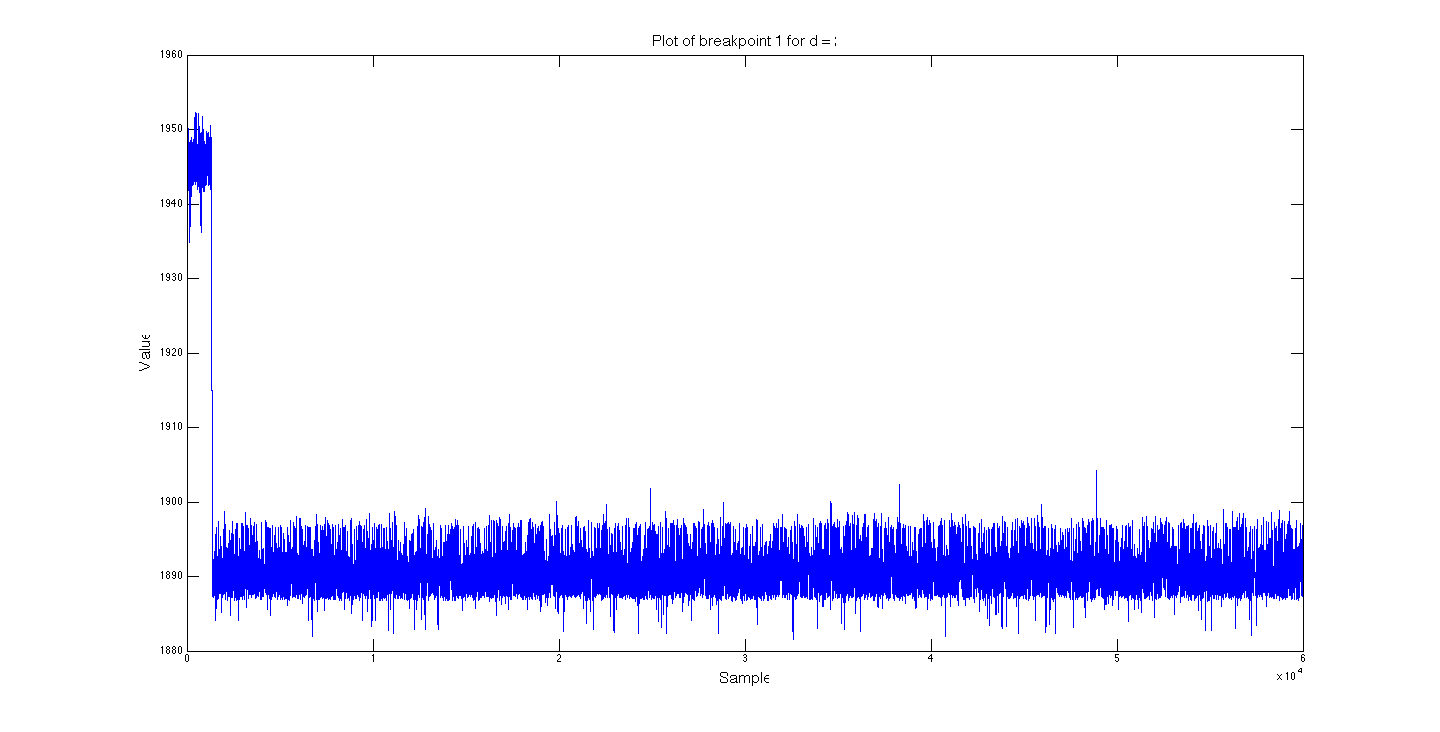
\includegraphics[scale=0.26]{./Figures/iburn.png}
\caption{Figure of the draws of $\boldsymbol{t}$}
\label{fig:burnin}
\end{figure}

As the figures shows, we have stationarity after about $M=3,000$ samples, meaning that our burn-in is reasonable. 

Here in assignment \textbf{c)} we investigate the behaviour of the chain for our posterior $f(\theta,\boldsymbol{\lambda},\boldsymbol{t}|\boldsymbol{\tau})$ for $1,2,3$ and 4 breakpoints in the data. We will show that the posterior of $\boldsymbol{t}$ for the intervals will be affected in various ways depending on the density for each interval.\\

For the remainder of this assignment, we analyze the number of breakpoints individually with $\beta = 1$ and $\rho = (0.05,\:,0.14,\:0.25,\:0.36)$.\\

\newpage
\subsubsection*{One Breakpoint}
If we divide the time period into two intervals we get that the breakpoint is located at $t\approx 1891$. Figure \ref{fig:bp1} shows where the location of the breakpoint is located relative to the dataset in order to get a better overview.

\begin{figure}[H]
\centering
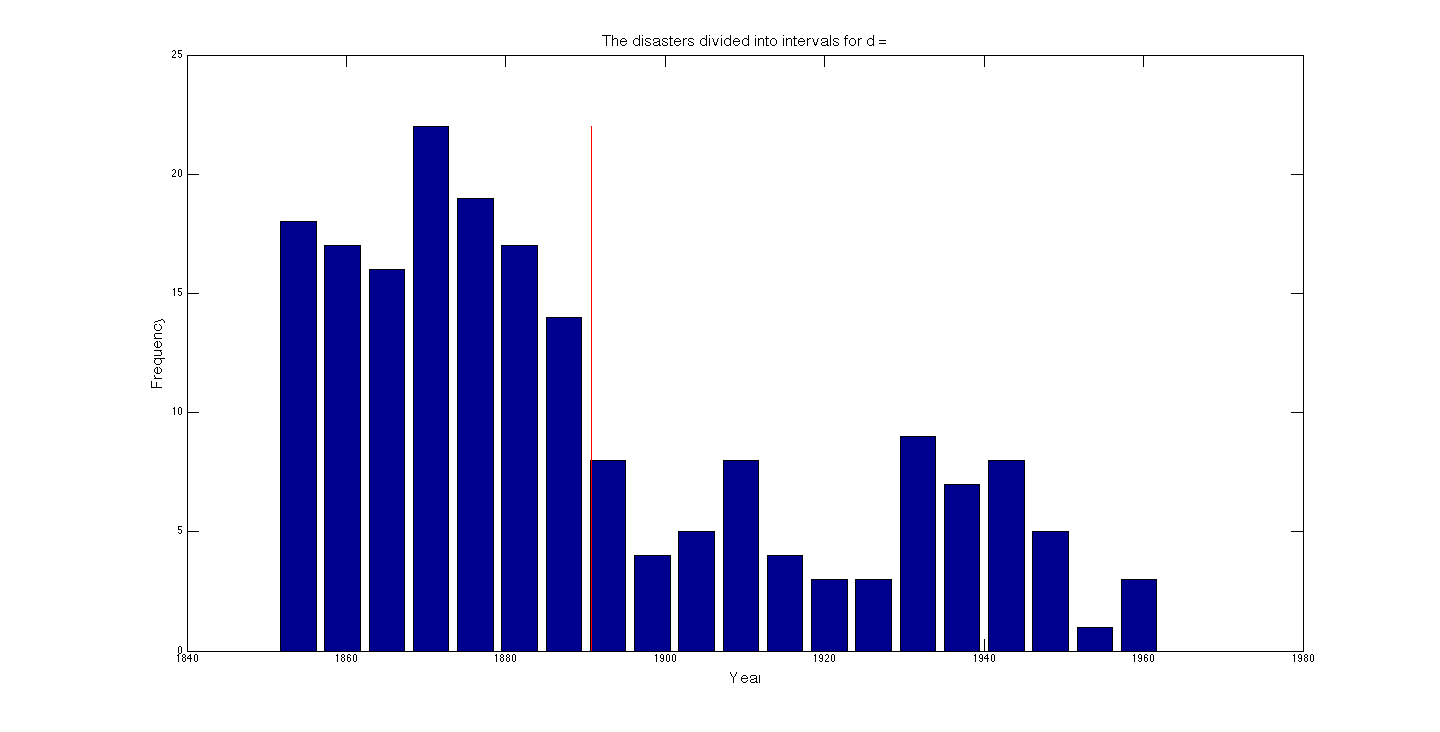
\includegraphics[scale=0.26]{./Figures/bp1.png}
\caption{Plot of where the breakpoint is located.}
\label{fig:bp1}
\end{figure}

In the introduction we said that the breakpoint should lie somewhere at the turn of the century, and as is seen in figure \ref{fig:bp1} we have a reasonable result as to where the breakpoint lies. \\ We now look at the histogram of the breakpoint in figure \ref{fig:tpost1}.

\begin{figure}[H]
\centering
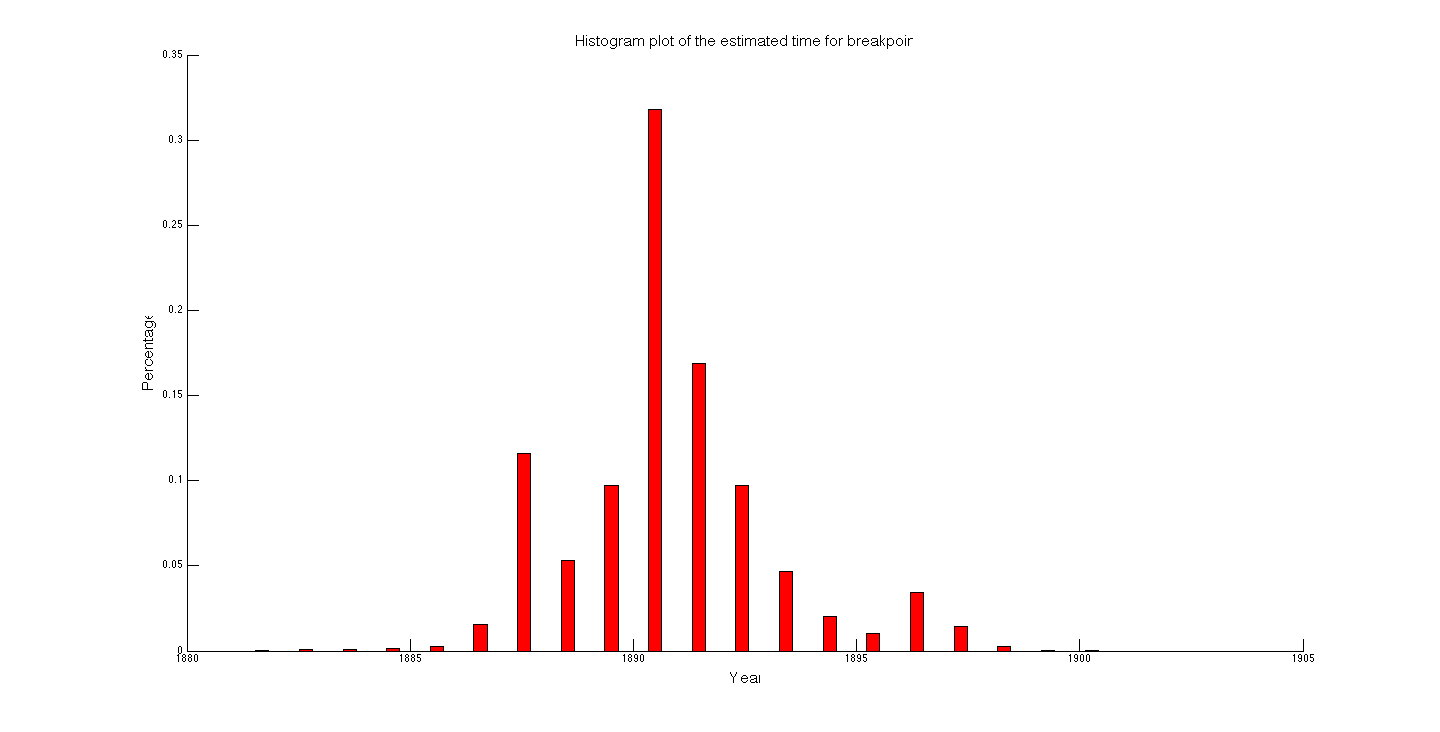
\includegraphics[scale=0.26]{./Figures/tpost1.png}
\caption{Histogram plot of the breakpoint.}
\label{fig:tpost1}
\end{figure}

As is seen in figure \ref{fig:tpost1}, the histogram is centered around 1891 with a small tail indicating a high accuracy in the estimation of the breakpoint. We visualize the draws from the posterior in figure \ref{fig:t1}.

\begin{figure}[H]
\centering
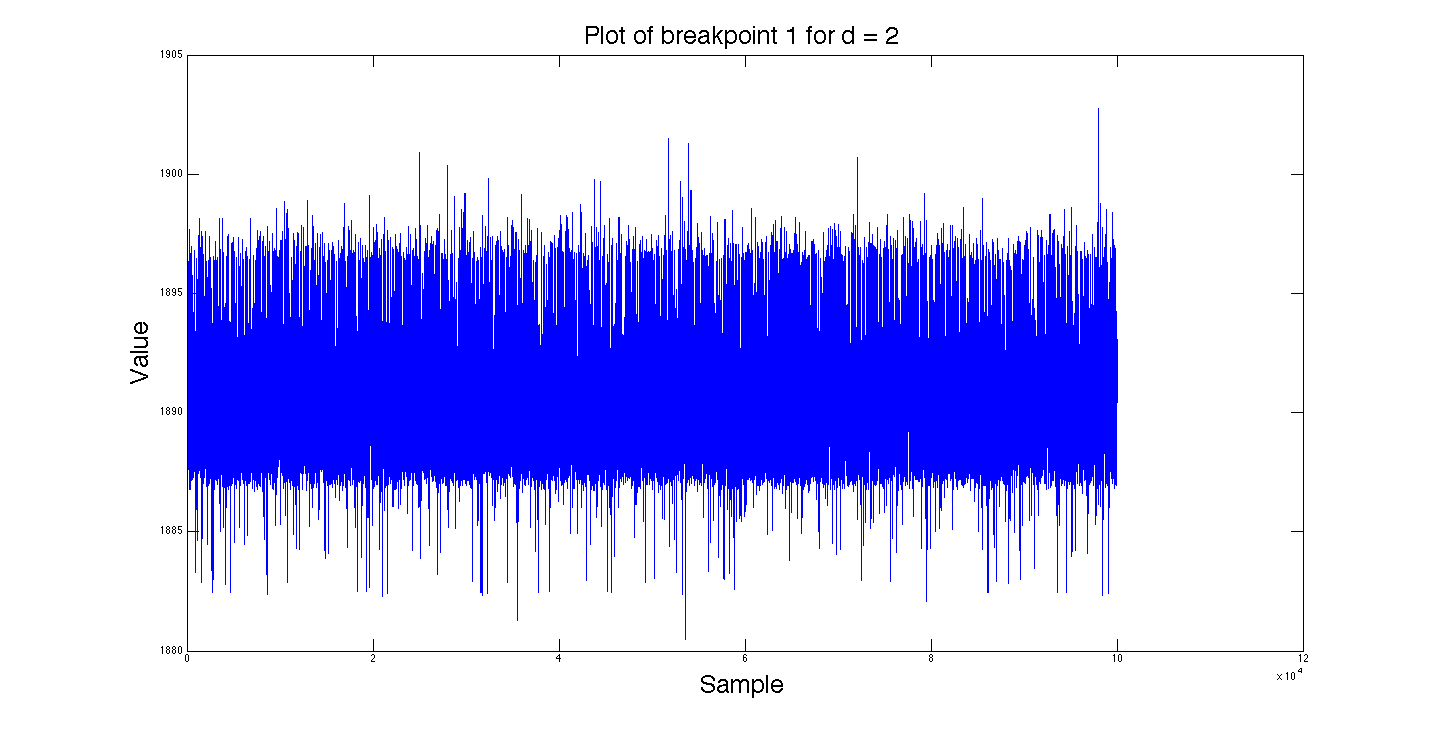
\includegraphics[scale=0.26]{./Figures/t1.png}
\caption{Visualization of the draws for the first breakpoint.}
\label{fig:t1}
\end{figure}

As is seen in the above figure the draws seem to be rather random and not depending on previous values.
We move on to investigate the behaviour of the intensities and see figure \ref{fig:lpost1}.

\begin{figure}[H]
\centering
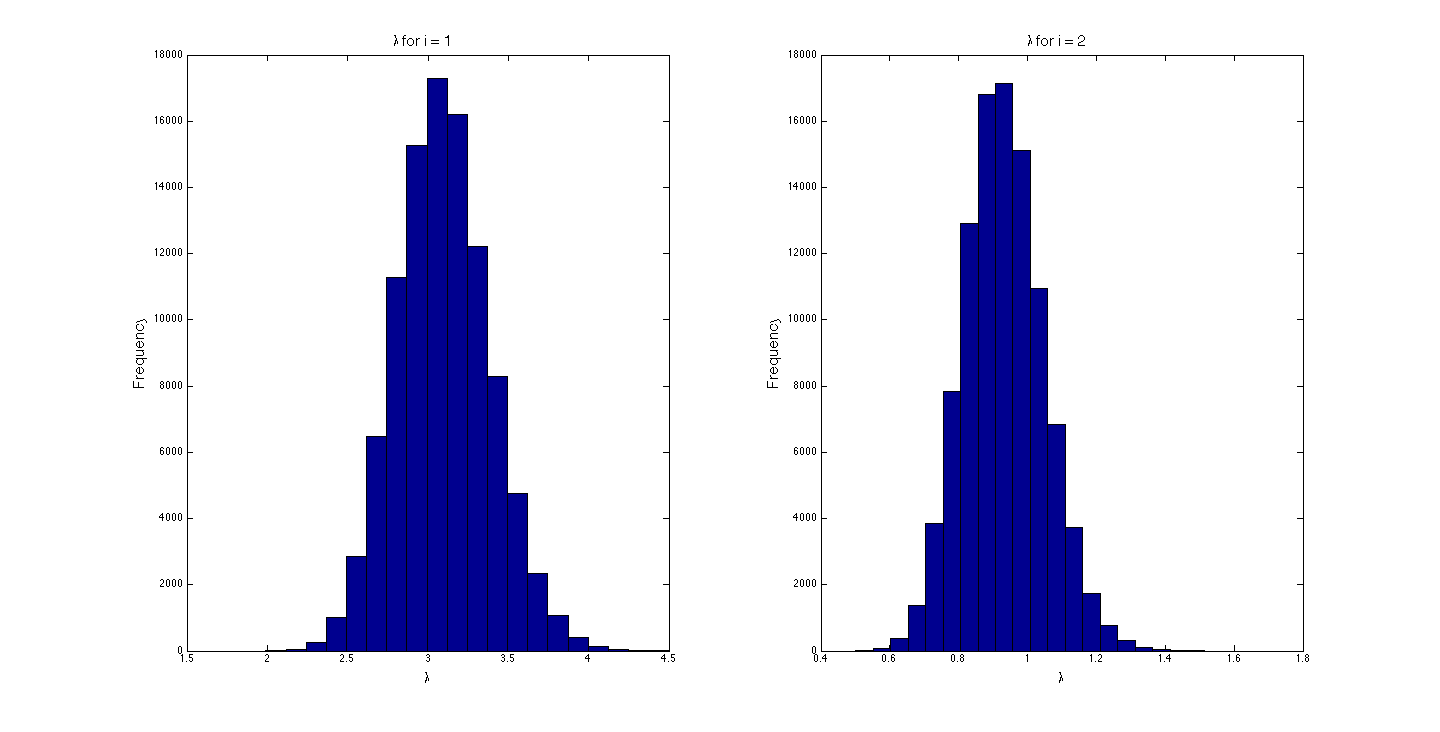
\includegraphics[scale=0.26]{./Figures/lpost1.png}
\caption{Histogram of the intensites of the two intervals.}
\label{fig:lpost1}
\end{figure}

The above figure suggests that the intensites both have a $\Gamma$--distribution where the first intensity is centered around $\approx 3.1$ disasters/year whereas the second intensity is centered around $\approx 0.91$ disasters/year, indicating a decrease of almost 70\%. \\ Finally we look at the histogram of $\theta$, which is seen in figure \ref{fig:thetapost1}.

\begin{figure}[H]
\centering
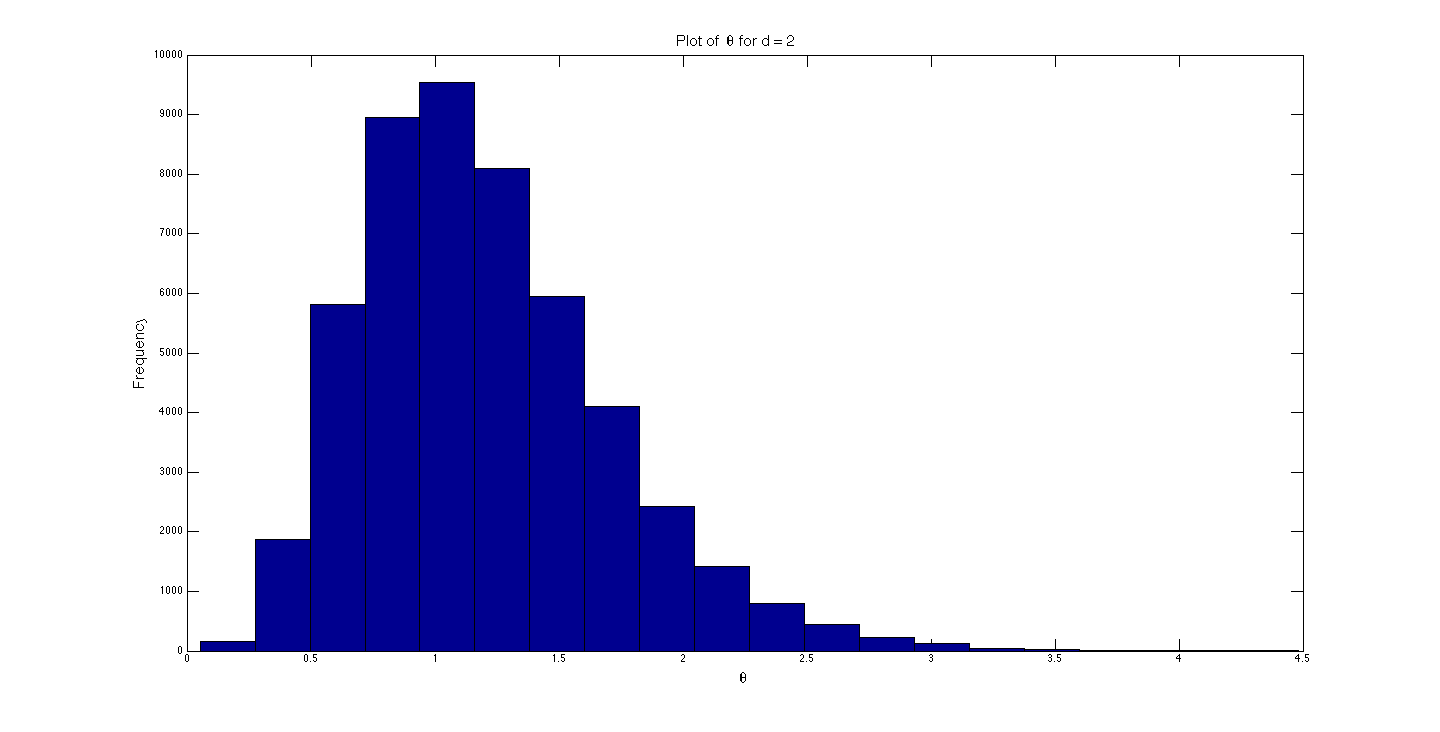
\includegraphics[scale=0.26]{./Figures/thetapost.png}
\caption{Histogram plot of $\theta$.}
\label{fig:thetapost1}
\end{figure}

Figure \ref{fig:thetapost1} is suggestive of a $\Gamma$--distribution centered around $\approx 1.2$. 

\subsubsection*{Two Breakpoints}

We now move on to investigate the behaviour of the chain for two breakpoints. As before, we begin by looking at the location of the breakpoints, which is seen in figure \ref{fig:bp2}.

\begin{figure}[H]
\centering
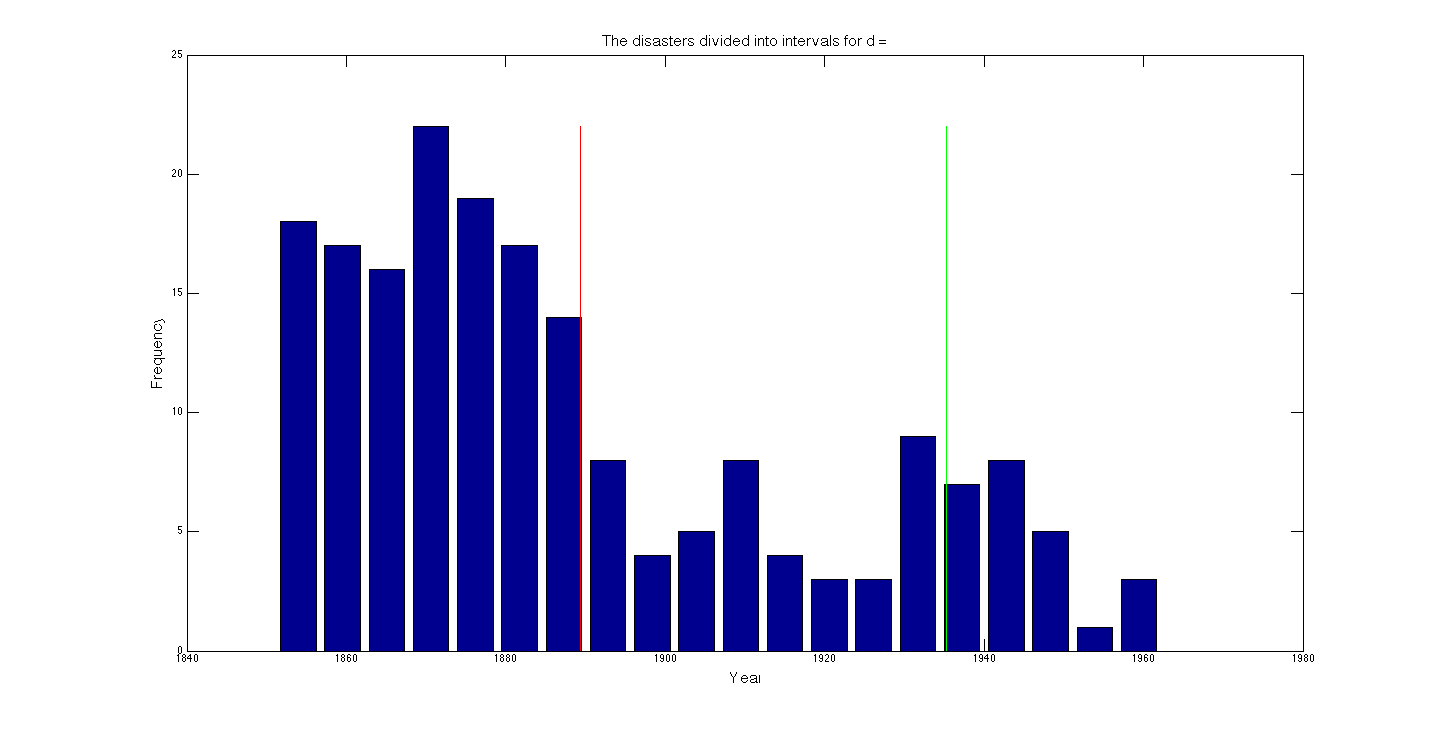
\includegraphics[scale=0.26]{./Figures/bp2.png}
\caption{Plot of where the breakpoints are located.}
\label{fig:bp2}
\end{figure}

As is seen in the above figure, the first breakpoint is almost located at the same time as before. This time it is $\approx 1890$ and the second breakpoint is located at $\approx 1937$. By looking at the figure, a more natural placement of the second breakpoint should be somewhere around 1930 since the change in intensity seems to occur there rather than at 1937. We move on to investigate the behaviour of the histogram of the breakpoints and look at figure \ref{fig:tpost2}.

\begin{figure}[H]
\centering
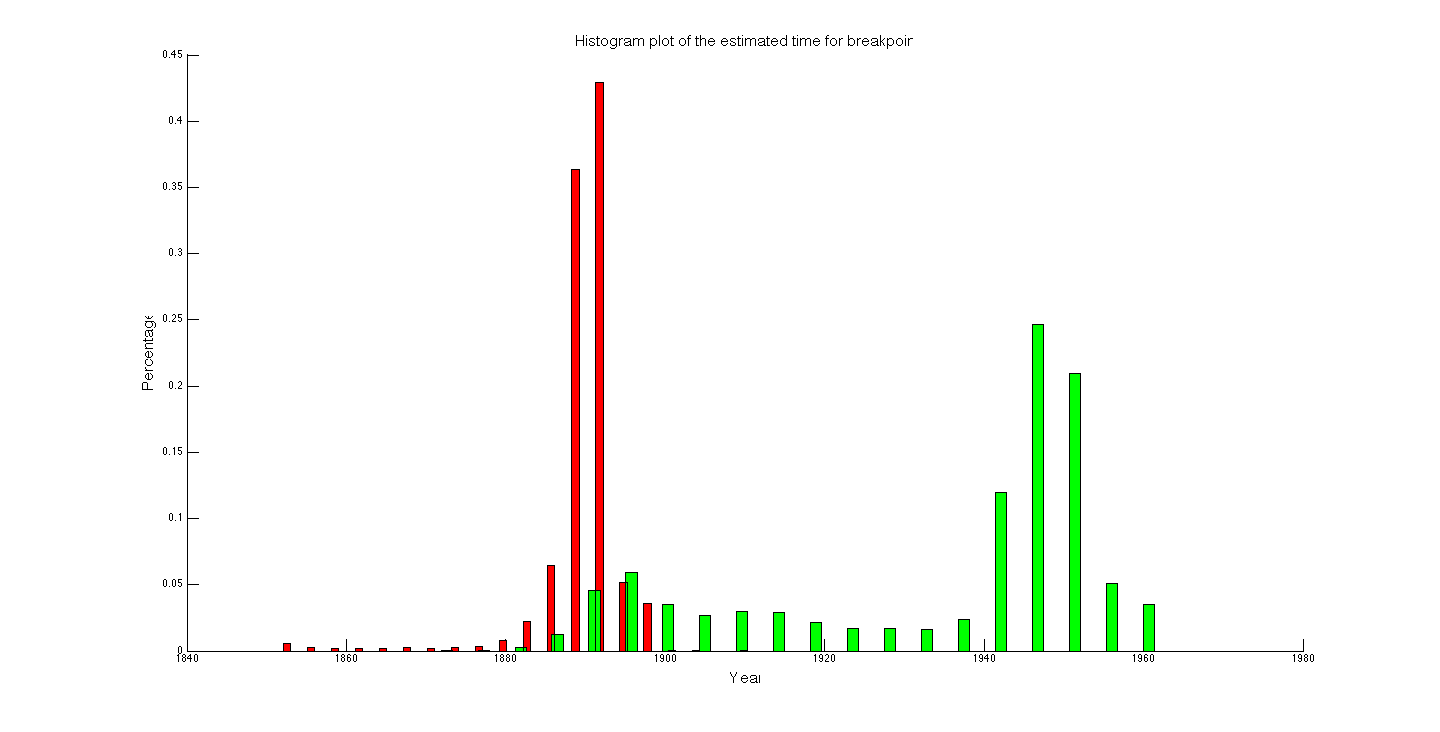
\includegraphics[scale=0.26]{./Figures/tpost2.png}
\caption{Histogram plot of the breakpoints.}
\label{fig:tpost2}
\end{figure}

As is seen in the above figure we have almost the same density as in figure \ref{fig:tpost1} for the first breakpoint, indicating a high accuracy of the results. Whereas we for the second breakpoint have rather large tails spanning almost the entire time period. This result is rather disappointing since we can expect to have a bad estimation of our second breakpoint. The samples that are drawn from the posterior are represented in figure \ref{fig:t2}.

\begin{figure}[H]
\centering
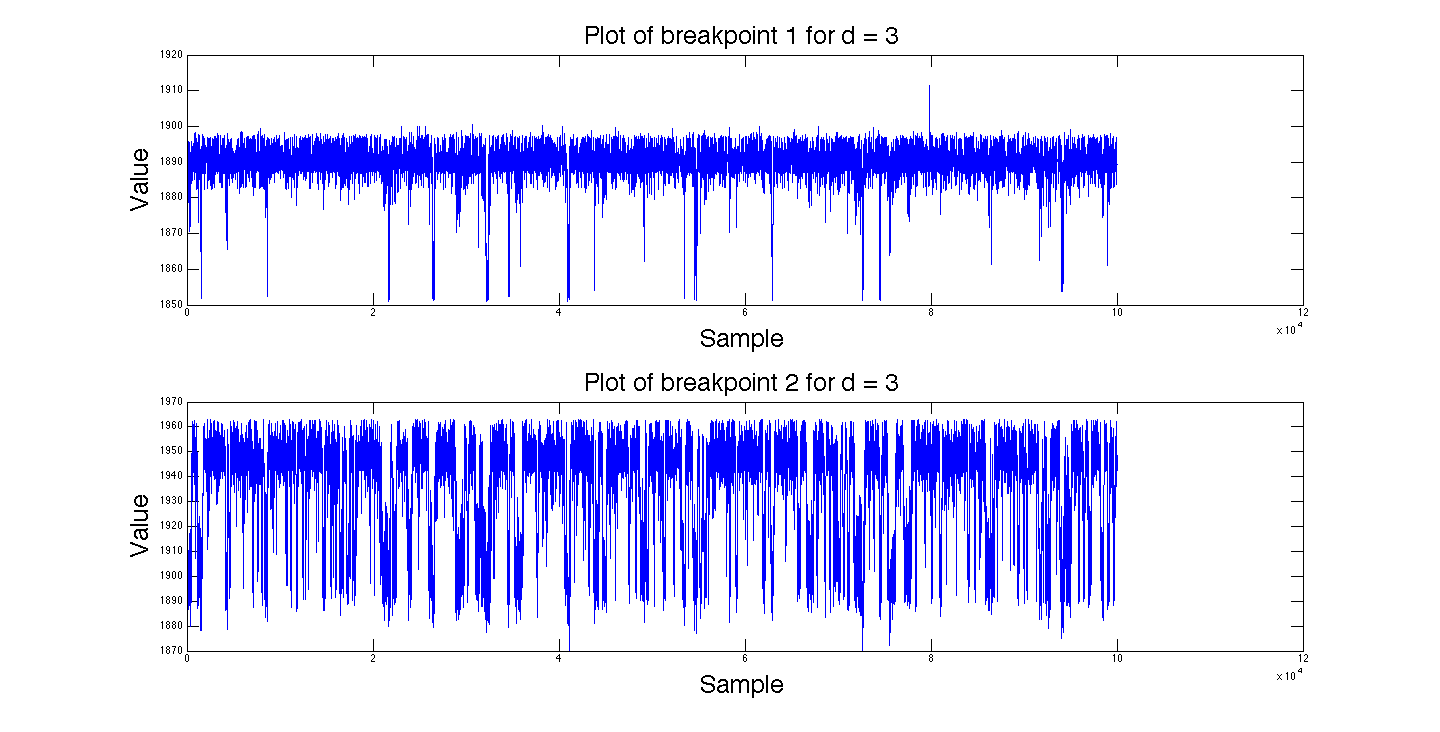
\includegraphics[scale=0.26]{./Figures/t2.png}
\caption{Visualization of the draws for both of the breakpoints.}
\label{fig:t2}
\end{figure}

As is seen in the figure above there is a small dependence of the draws, which could result in bad estimatations. \\
We turn our eyes toward the histograms of the intensties in figure \ref{fig:lpost2}.

\begin{figure}[H]
\centering
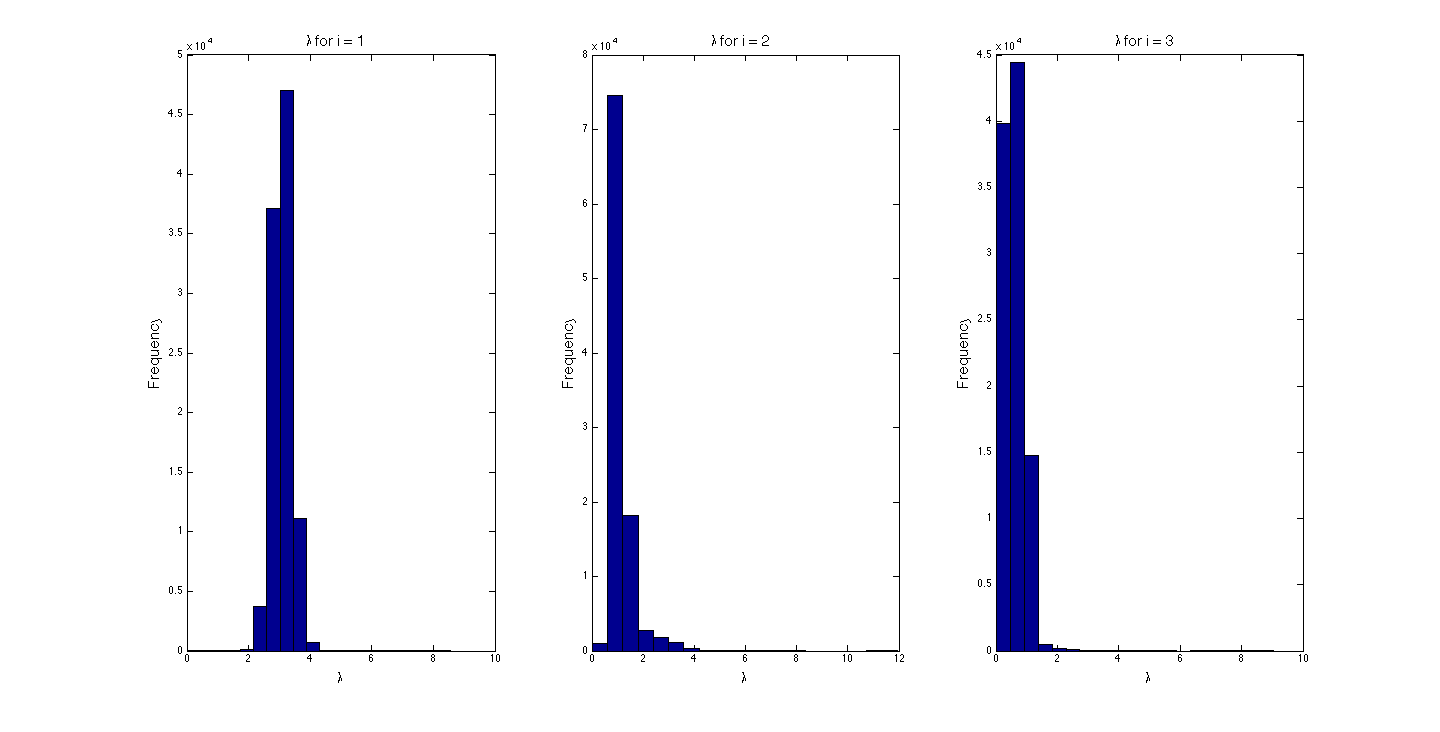
\includegraphics[scale=0.26]{./Figures/lpost2.png}
\caption{Histogram plot of the intensities.}
\label{fig:lpost2}
\end{figure}

By looking at the above figures we see that all of the intensities exhibit a $\Gamma$--distribution where they are centered around the values given by $\boldsymbol{\lambda} \approx (3.1,1.2,0.6)$. Since the first intensity and the first breakpoint are approximately the same as for one breakpoint we can assume that the "correct" breakpoint is somewhere between 1890--1891. \\ We finally look at the histogram of $\theta$ in figure \ref{fig:thetapost2}.

\begin{figure}[H]
\centering
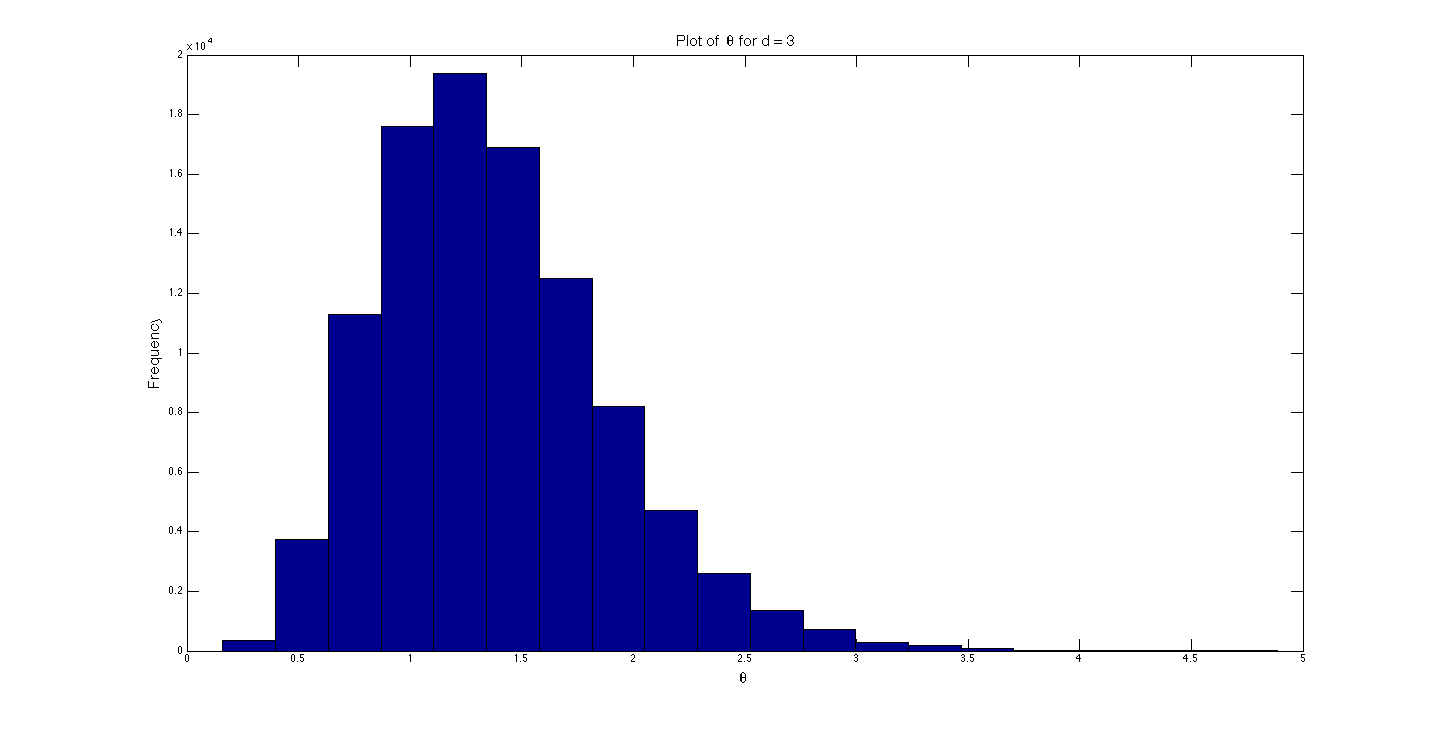
\includegraphics[scale=0.26]{./Figures/thetapost2.png}
\caption{Histogram plot of $\theta$.}
\label{fig:thetapost2}
\end{figure}

The histogram is highly indicative of $\Gamma$--distribution centered around $\approx 1.38$.

\newpage
\subsubsection*{Three breakpoints}
As in the previous sections we begin with investigating where the breakpoints are located, which is seen in figure \ref{fig:bp3}.

\begin{figure}[H]
\centering
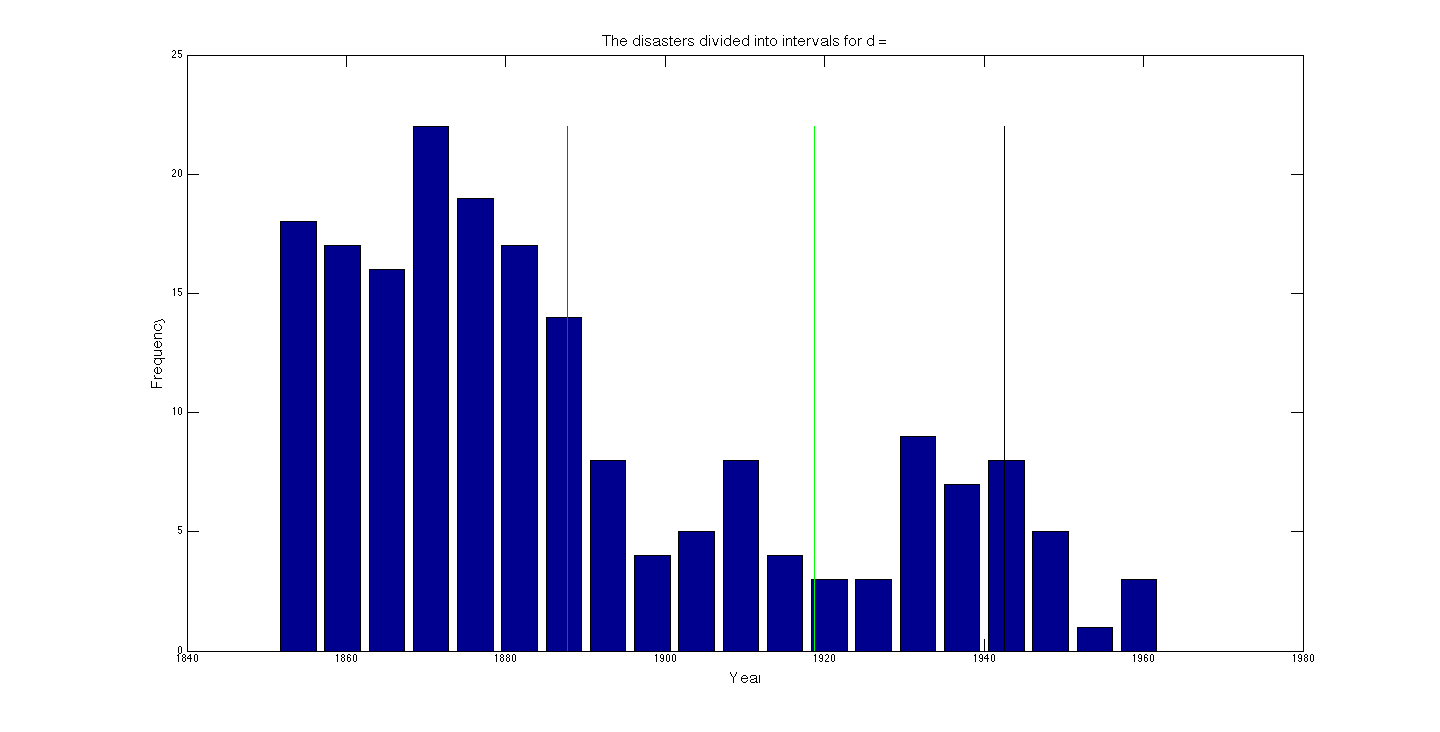
\includegraphics[scale=0.26]{./Figures/bp3.png}
\caption{Plot of where the breakpoints are located.}
\label{fig:bp3}
\end{figure}

From the above figure we see that the first breakpoint has moved to 1884 and the two other breakpoints are located around 1911 and 1942. It is difficult to comment on these locations since more than two breakpoints seem superflous. We thus look at the histogram plot of the breakpoints in figure \ref{fig:tpost3}.

\begin{figure}[H]
\centering
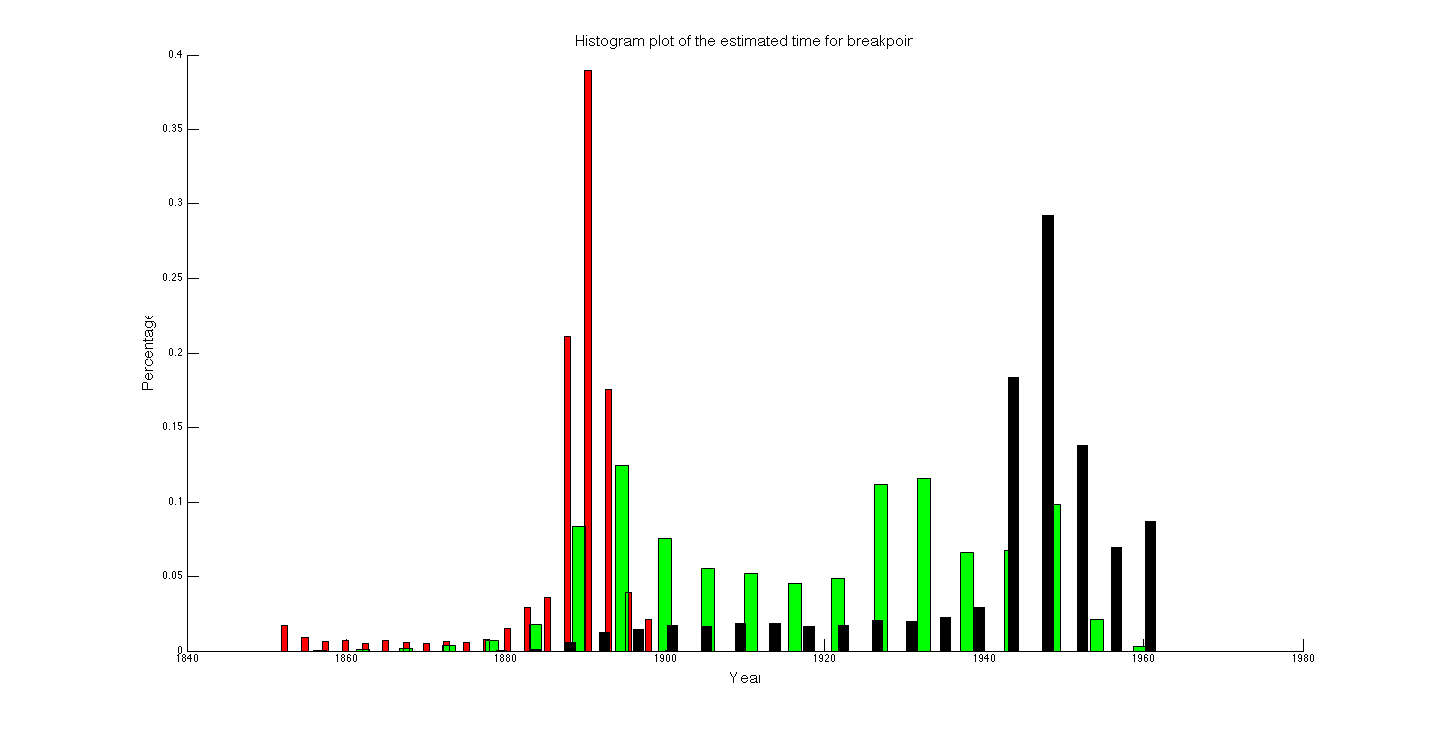
\includegraphics[scale=0.26]{./Figures/tpost3.png}
\caption{Histogram plot the breakpoints.}
\label{fig:tpost3}
\end{figure}

From the above figure we see that the histogram of the first breakpoint has a tiny tail to the left of the center suggesting a good estimation. The histogram of the second breakpoint is bad since we cannot distinguish a center of the density, which suggests that we will have a bad estimation in the breakpoint, it also spans over a large interval. The third histogram has almost the same density as that of the first density. It has a centered value with a small tail to the left, but most of the mass is located around the center. Here we can also note that it spans across a large interval. \\ We now investigate the behaviour of the draws from this posterior, which are visualized in figure \ref{fig:t3}.

\begin{figure}[H]
\centering
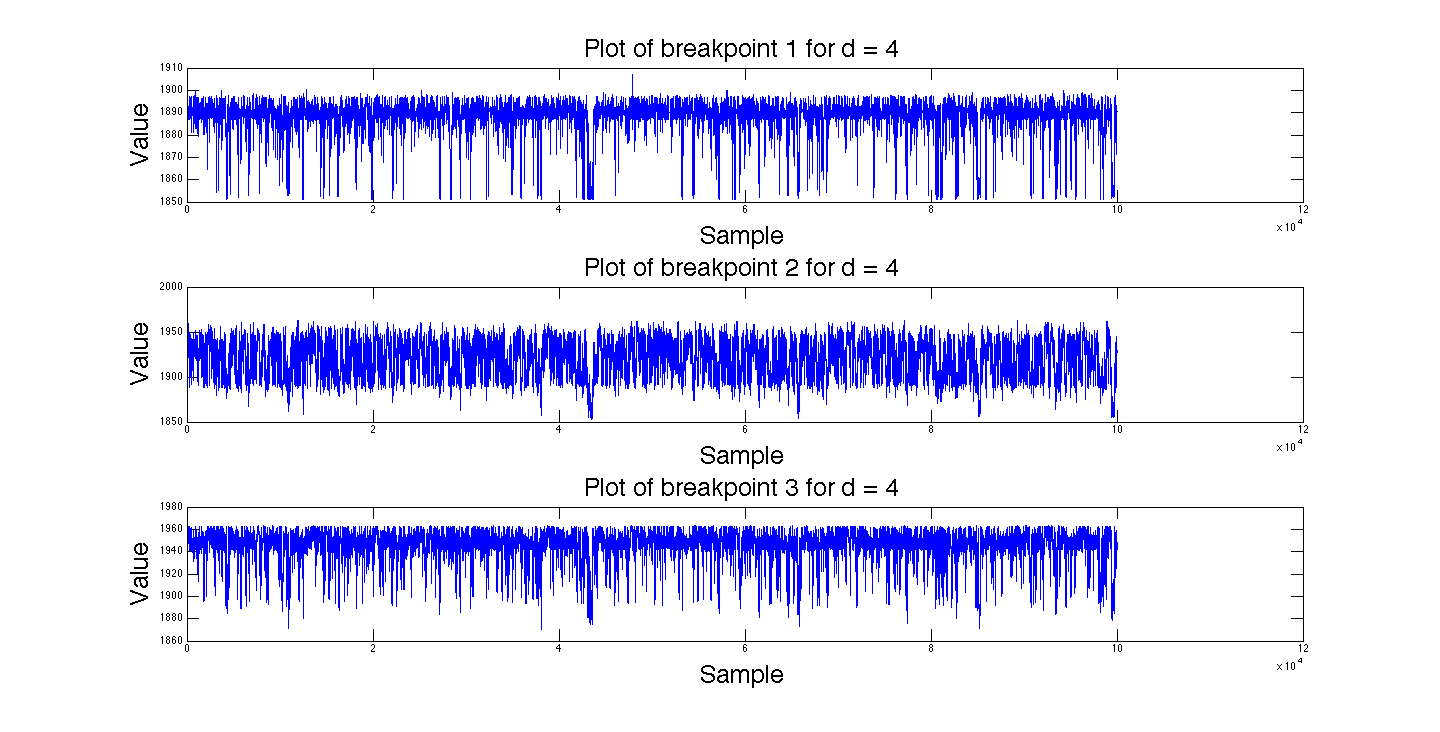
\includegraphics[scale=0.26]{./Figures/t3.png}
\caption{Visualization of the draws for both of the breakpoints.}
\label{fig:t3}
\end{figure}

As we can see in the above figure we have little dependence between the different draws. \\ We now move on to look at the histograms of the intensities.

\begin{figure}[H]
\centering
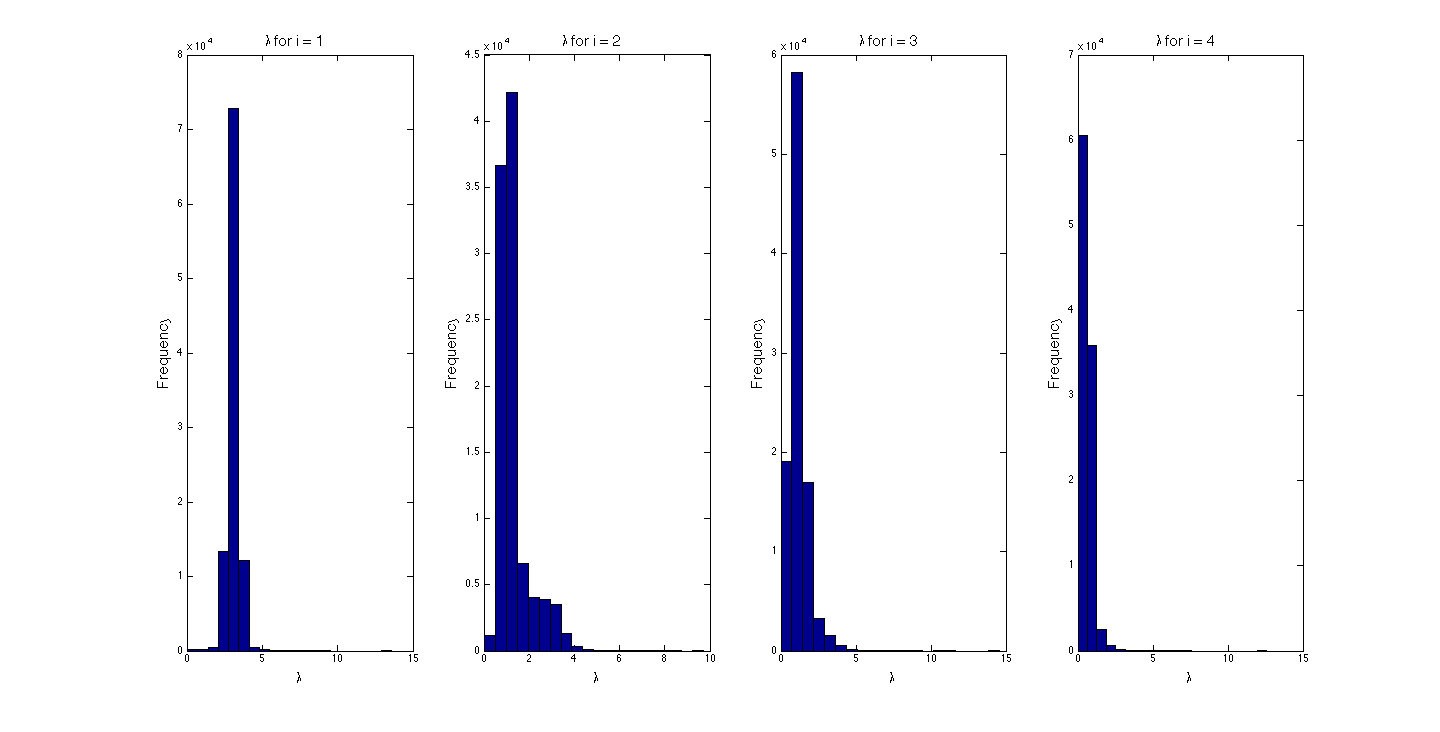
\includegraphics[scale=0.26]{./Figures/lpost3.png}
\caption{Histogram plots of the intensities.}
\label{fig:lpost3}
\end{figure}

From the above figure it is possible to discern a $\Gamma$--distribution for the distributions. The intensity for the first interval is still $\approx 3.1$. Lastly, we look at the histogram plot of $\theta$.

\begin{figure}[H]
\centering
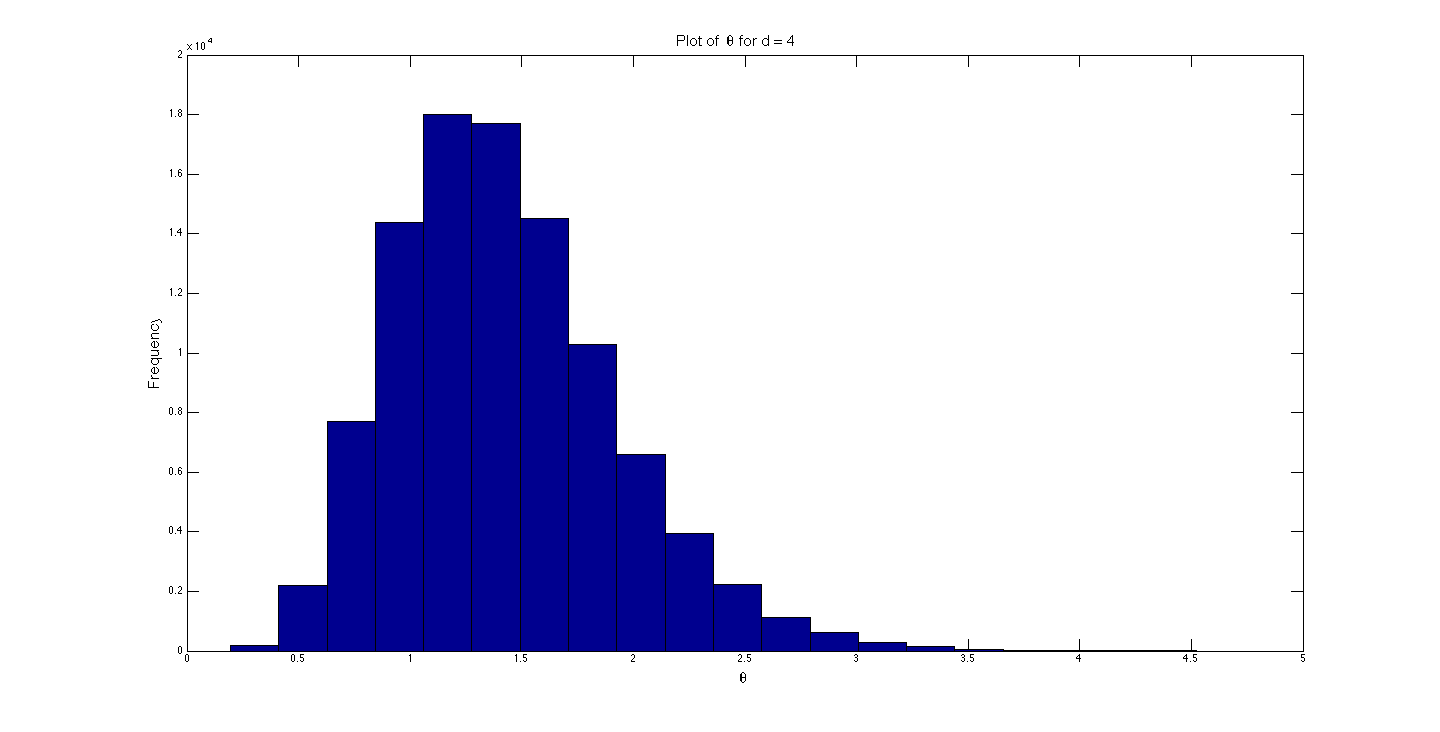
\includegraphics[scale=0.26]{./Figures/thetapost3.png}
\caption{Histogram plot of $\theta$.}
\label{fig:thetapost3}
\end{figure}

From the figure above, we see that $\theta$ still has the $\Gamma$--distribution but centered around 1.4.
\newpage
\subsubsection*{Four Breakpoints}

Finally, we investigate the behaviour using four breakpoints. We begin by looking at the location of the breakpoints as seen in figure \ref{fig:bp4}.

\begin{figure}[H]
\centering
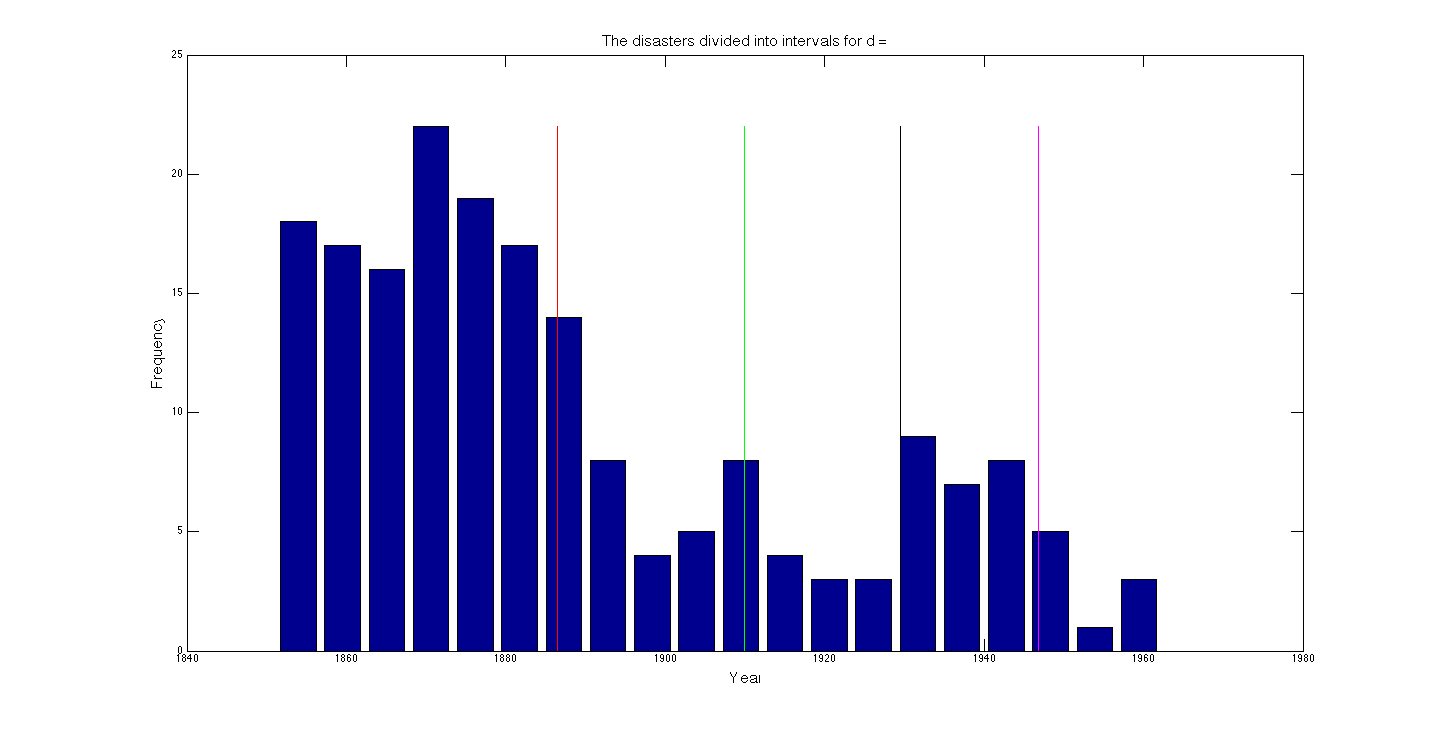
\includegraphics[scale=0.26]{./Figures/bp4.png}
\caption{Plot of where the breakpoints are located.}
\label{fig:bp4}
\end{figure}

From the above figure we see that the first breakpoint again has moved, but this time it did not move that far from the breakpoint suggested using only one breakpoint. It is now located around 1887. The second breakpoint is located around 1911, which is close to the second breakpoint when using three breakpoints. As in the previous section, it is difficult to say anything about the placement of the breakpoints since more than two seem superflous. We instead look at the histogram plot over the breakpoints.

\begin{figure}[H]
\centering
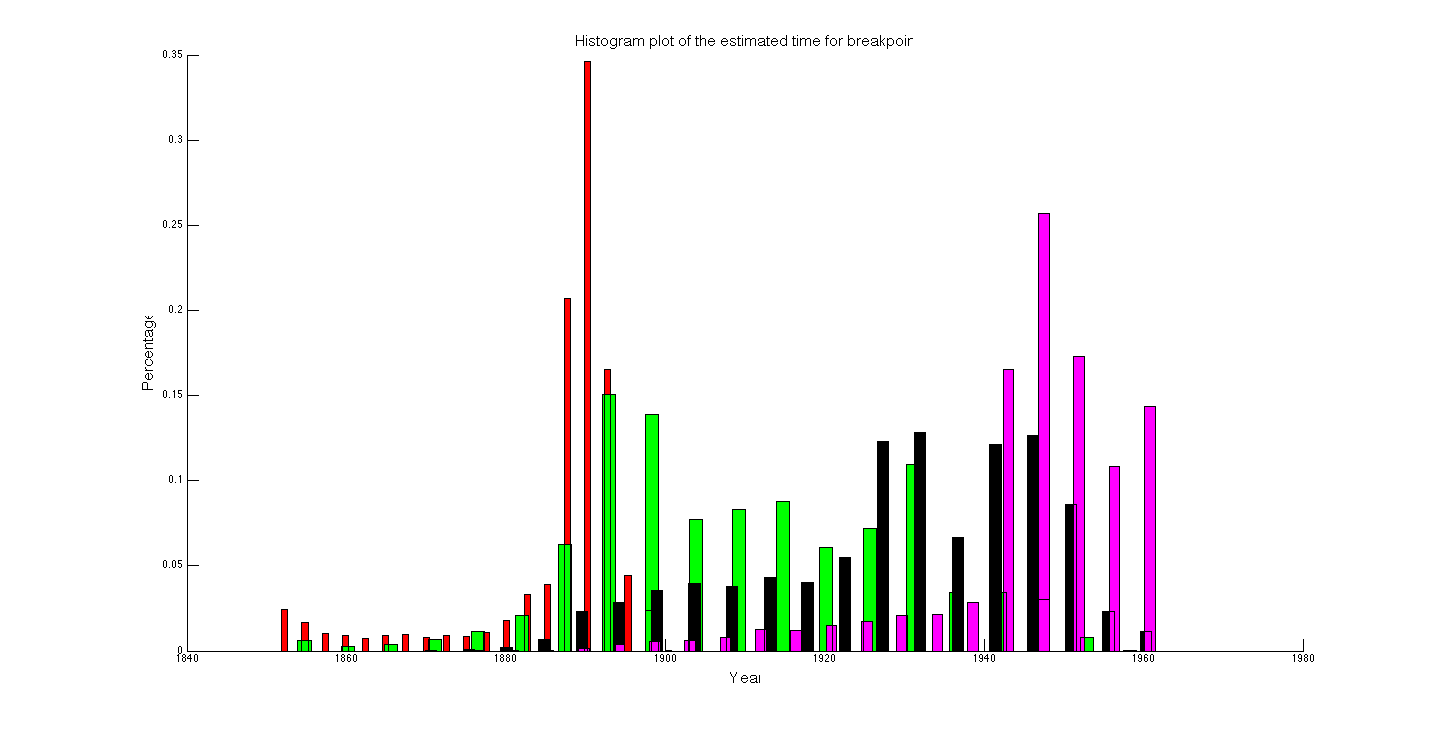
\includegraphics[scale=0.26]{./Figures/tpost4.png}
\caption{Histogram plot the breakpoints.}
\label{fig:tpost4}
\end{figure}

From the histogram above we can see that the first breakpoint behaves as previously around 1887. The second breakpoint also spans across a large interval, indicating a bad estimate. The third breakpoint has its mean around 1929, but spans across a large interval and is approximately uniform, indicating a bad estimate. The fourth breakpoint has its mean around 1948 and has almost the same distribution as the first, but with less frequency, here we can again conclude that this breakpoint could be good. We now move on to the draws of the breakpoints.

\begin{figure}[H]
\centering
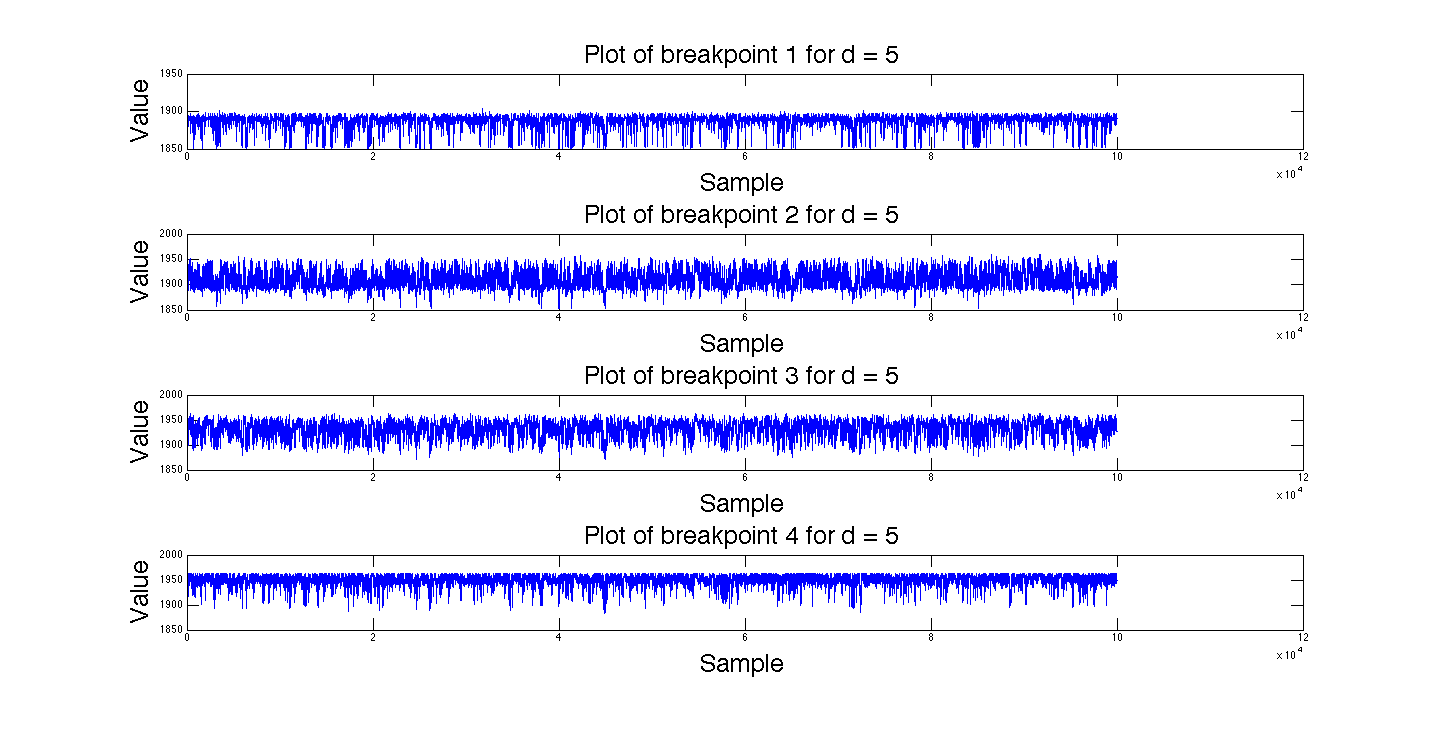
\includegraphics[scale=0.26]{./Figures/t4.png}
\caption{Visualization of the draws for both of the breakpoints.}
\label{fig:t4}
\end{figure}


As we can see in the above figure we have little dependence between the different drawshere as well. This indicates that our values of $\rho$ gives the draws a random behaviour.. \\ We now move on to look at the histograms of the intensities.

\begin{figure}[H]
\centering
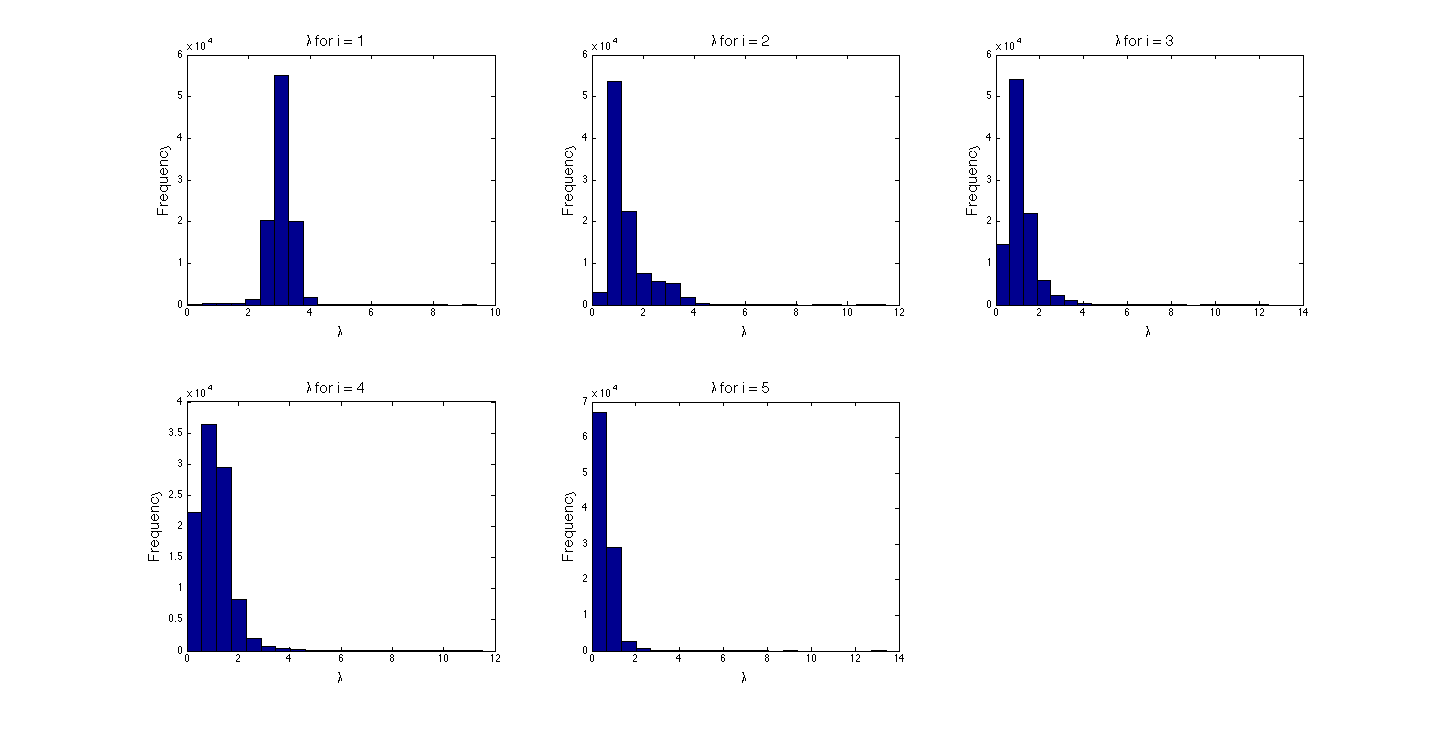
\includegraphics[scale=0.26]{./Figures/lpost4.png}
\caption{Histogram plots of the intensities.}
\label{fig:lpost4}
\end{figure}

From the above figure it is possible to discern a $\Gamma$--distribution for the distributions. The intensity for the first interval is still $\approx 3.1$. Lastly, we look at the histogram plot of $\theta$.

\begin{figure}[H]
\centering
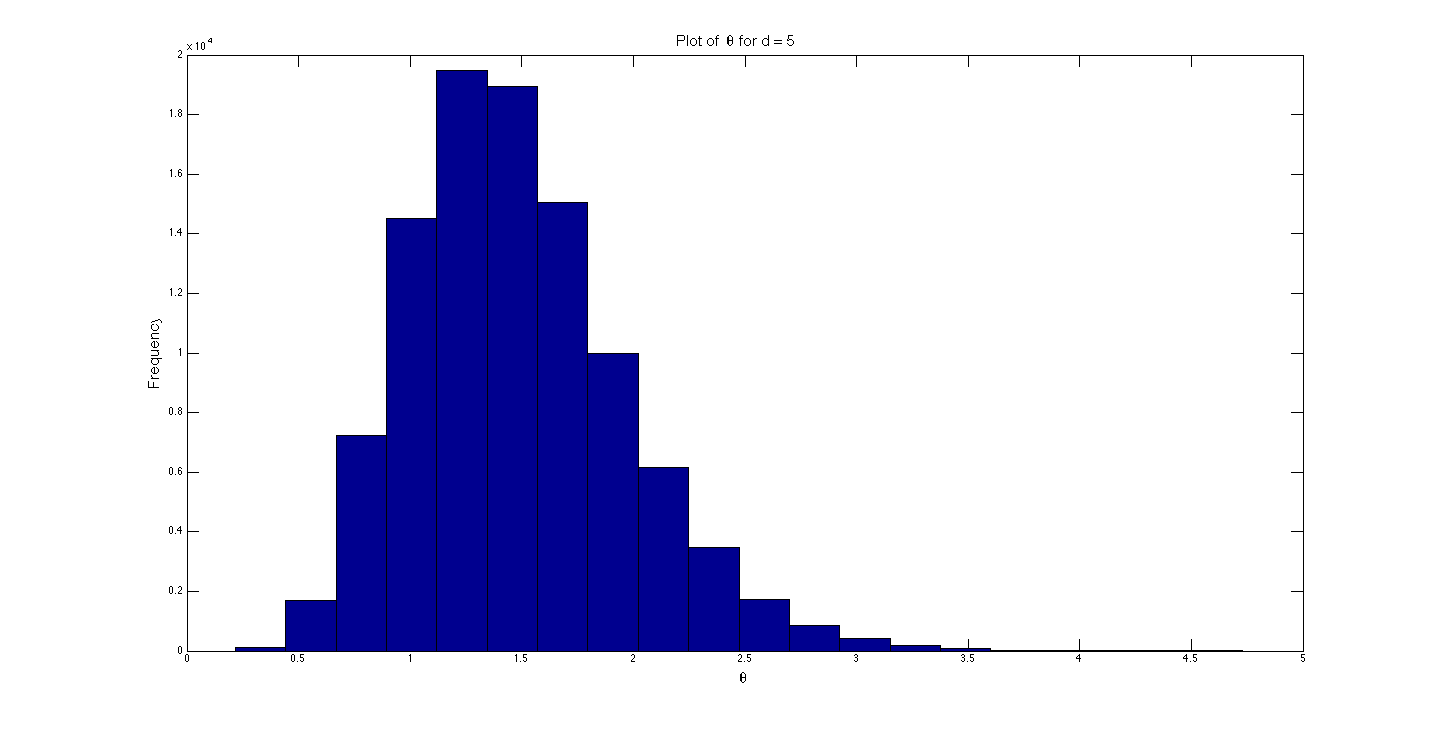
\includegraphics[scale=0.26]{./Figures/thetapost4.png}
\caption{Histogram plot of $\theta$.}
\label{fig:thetapost4}
\end{figure}

The histogram for $\theta$ is clearly has a $\Gamma$--distribution with center 1.46. \\ \\
We gather all of the breakpoints and intensities in table\ref{tablez} such as to get some overview, 


\begin{table}[H]
\begin{tabular}{|c|c|c|c|c|}
\hline
Breakpoints & 1 & 2 & 3 & 4 \\ \hline
$\boldsymbol{t}$ & 1891 & (1890,\:1937) & (1884,\:1911,\:1942) & (1889,\:1915,\:1933,\:1950) \\ \hline
$\boldsymbol{\lambda}$ & (3.1,\:0.9) & (3.1,\:1.2,\:0.6)  & (3.1,\:1.5,\:1.3,\:0.6)  & (3.1,\:1.3,\:1.1,\:1.2,\:0.6) \\ \hline
$\theta$ & 1.1995 & 1.3441 & 1.3536 & 1.408 \\ \hline
\end{tabular}
\label{tablez}
\end{table}

%These plots illustrate the expected breakpoints and therefore the associated intervals. As such we can evaluate if the interval data exhibit that of a gamma-distribution. We have illustrated the histograms in figures \ref{fig:tpost} of the $\boldsymbol{t}$-posteriors for each breakpoint, in order to investigate the probability of our breakpoint estimates. To also ensure that our prior $\theta$ has been established correctly, we here plot the histogram of $\theta$ indicating that it is of $\Gamma$-distributed character. The obtained $\theta$s and $\boldsymbol{\lambda}$ from our hyperprior is plotted in the figures \ref{fig:thetapost} and \ref{fig:lpost} respectively


%When sampling from the $f(\theta|\boldsymbol{\tau},\boldsymbol{\lambda},\boldsymbol{t})$ the histogram plot of the different $\theta$s. The same distribution occured for each case, as seen in the plots above. Hence we have only plotted two cases.
%Lambda posteriors


If the figures show a strong convergence towards an estimated value, we can assume that our approximation is good, i.e. when the histogram plots are localized around one value. Whenever a shift occurs we have a new Po-distribution in the data. Looking at the left figure in figure \ref{fig:bp2} we can easily see that the breakpoints is centered around 1891 with a small tail, thus indicating that the approximation is valid. By also looking at figure \ref{fig:bp1} we can easily see that there is a change in intensity at 1891. \\

When the data has been divided with two breakpoints, as seen in the right figure of figure \ref{fig:tpost2}. It is seen that the first breakpoint basically has the same distribution as only using one breakpoint, i.e. small tails and centered around 1891. However, the second breakpoint is centered around 1945 where most of the mass is allocated around this value. It is however also noted that there is a heavy tail of the distribution spanning across 50 years. \\

The left figure of figure \ref{fig:tpost3} shows the histograms of the three breakpoints. It is seen the the first breakpoint corresponds to almost the same previous values, i.e. centered around 1890, but one can note that there is a tail to the left. The second breakpoint is the most interesting, since there seems to be two centers, one in 1890 and one in 1940. Indicating an uncertainty in the estimation as the Monte Carlo approximation will be highly affected. The third breakpoint has the same distribution as the first and is centered around 1944. \\

\subsubsection*{Summary}
From the previous analysis we can deduce that if we would divide the disasters into blocks with different intensities, we would use one breakpoint at the year 1891. Giving the intensities of the disasters as the figures show in \ref{fig:lpost1}. The intensity between the years 1851--1891 would be $\lambda_1 \approx 3.1$ disasters per year and the intensity between 1891--1963 would be $\lambda \approx 0.9$. It can also be concluded that the chosen values for $\rho$ give a random and independent behaviour of the draws for the kernel of the MH algorithm. 


\subsection*{d)}
In this exercise, we are supposed to investigate the sensitivity of the posteriors when we vary the hyperparameter $\beta$. Since we do not have a "correct" answer for all of the parameters, we will investigate the sensitivity by calculating the variance of the parameters when drawing from the posteriors several times. We will investigate what happens for $\beta = 0, 1, 5, 20$ with a constant $\rho = 0.14$. In order to investigate the sensitivity we chose simulate the chain 100 times for each value of $\beta$ with a burn--in of 10,000 samples, 25,000 samples and two breakpoints. The variance for each of the parameters was then calculated and are found in the table below. Each of the columns represent the variance of that parameter.

\begin{table}[H]
\centering
\begin{tabular}{|c|c|c|c|c|c|c|}
\hline
Parameters & $\theta$ & $t_2$ & $t_3$ & $\lambda_1$ & $\lambda_2$ & $\lambda_3$  \\ \hline
$\beta = 0$ & $1.7\cdot 10^{-4}$ & 0.14 & 4.21 & $1.5 \cdot 10^{-5}$ & $8.3 \cdot 10^{-4}$ & $3.6\cdot 10^{-4}$ \\ \hline
$\beta = 1$ & $1.2\cdot 10^{-4}$ & 0.16 & 5.23 & $1.3 \cdot 10^{-5}$ & 0.0012 & $4.2 \cdot 10^{-4}$ \\ \hline
$\beta = 5$ & $3.3 \cdot 10^{-5}$ & 0.43 & 7.44 & $4.58 \cdot 10^{-5}$ & 0.0031 & $4.6 \cdot 10^{-4}$ \\ \hline
$\beta = 20$ & $2.23 \cdot 10^{-6}$ & 0.72 & 7.55 & $5.9 \cdot 10^{-4}$ & 0.0068 & $9.8 \cdot 10^{-4}$ \\ \hline
\end{tabular}
\end{table}

As we can see in the above table we have the lowest overall variance of the parameters for $\beta = 0$ followed up by $\beta = 1$ etc. This implies that the estimates will be less prone to vary the lower the value of $\beta$ is. One thing to note is that the variance of $\theta$ is improved the greater the value of $\beta$ where as the other parameters' variances are increased. One must thus use a sufficienlty large enough $\beta$ in order to get "accurate" values of $\theta$ where as you need a small enough value to get accurate values of the parameters. \\ \\ It should be noted that we only simulated the chain 100 times, which might not be enough in order to get stable results. But since we used 25,000 samples for each simulation we consider these results to be somewhat accurate. We were unfortuneately not able to simulate more since the simulations are rather slow, but we simulated the chain a couple of times for lower amount of times and got almost the same results.

%In this exercise we are supposed to investigate the behaviour of the chain when we vary the hyperparameter $\beta$. We investigate what happens for $\beta = 20$ and $\beta = 0$. When we use $\beta = 20$ we get very varying estimations of the breakpoints from one simulation to another, whereas the intensities and $\theta$ are somewhat consequent. The estimations of $\theta$ and the intensities are relatively constant. Thus for large values of $\beta$ the breakpoints are effected. \\
%\\
%However, if we set $\beta = 0$ the estimations are consistent in between simulations, meaning that we do not get results that vary notably between simulations. The results are basically the same as in \textbf{c)}, but the estimation of the first breakpoint when using three breakpoints is more "exact" in the sense that it sets the first breakpoint to $\approx 1890$. \\ The conclusion is that the posteriors are sensitive if one sets the hyperparameter to be too big. Whereas the posteriors become less prone to instability for small values of $\beta$, but not necessarily more correct. It is thus important not to set $\beta$ to be too big.



\subsection*{e)}
Here we will investigate the mixing and the posteriors in the proposal distribution. From the relation of $R$ in the definition. We note that $R$ depends both on $\rho$ and $t_{i+1}-t_{i-1}$. One can realize first that $R$ will be calculated for each breakpoint, hence an increase of breakpoints used, a decrease of the value of the differences will occur. We therefore need to increase $\rho$ accordingly. \\
\\
We know that $\rho$ will effect our sample space. Therefore if we choose $\rho$ for values 
\[ || \rho || > 0 + C, \quad \text{for} \quad C>> 0 \] 
indicates that we will consider a large portion of the sample space, in our case $X\in\mathbb{R}$. This in turn will only generate rejected samples, since we are almost 100\% outside of the our desired sample space. However, if $\rho=0$ or close to $0$, 
\[ || \rho ||+ \epsilon \geq 0,  \quad \text{for} \quad \epsilon \geq 0 \] 
we do not sample outside of the proposed distribution, meaning that we will only end up in the proposed values and again reject most of the sampled values. \\
\\
We know that $\rho$ must help to enclose the desired sample space. Since we know from the argumentation above, $\rho$ must be small and large enough but also depend on the breakpoints. Below in figures \ref{fig:fixrho1} and \ref{fig:fixrho4} are plots of the mixing for $\boldsymbol{t}$ with a fixed $\rho$. \\
\\
\begin{figure}[H]
  \centering
\begin{minipage}{1\textwidth}
    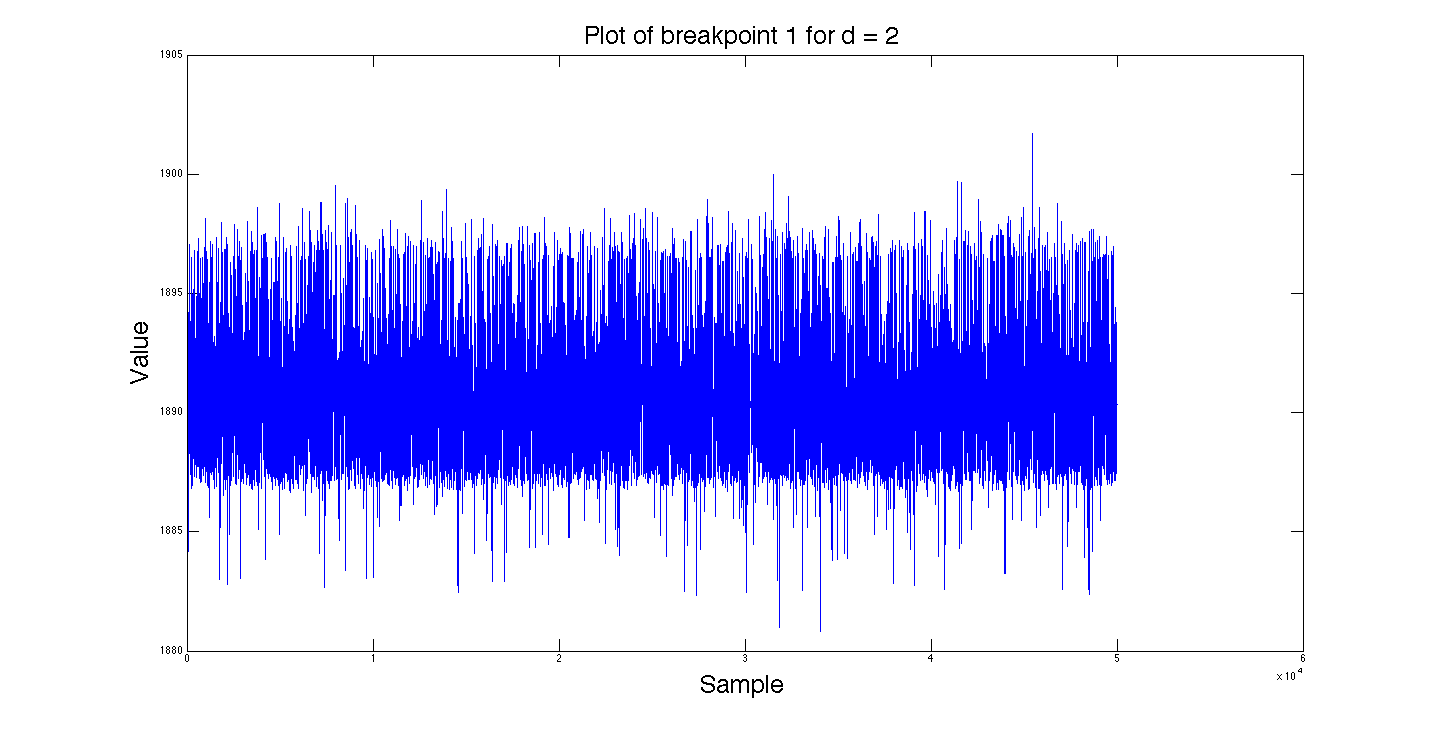
\includegraphics[scale=0.28]{./Figures/fixrho1.png}
  \label{fig:fixrho1}
\end{minipage}
%
\begin{minipage}{1\textwidth}
    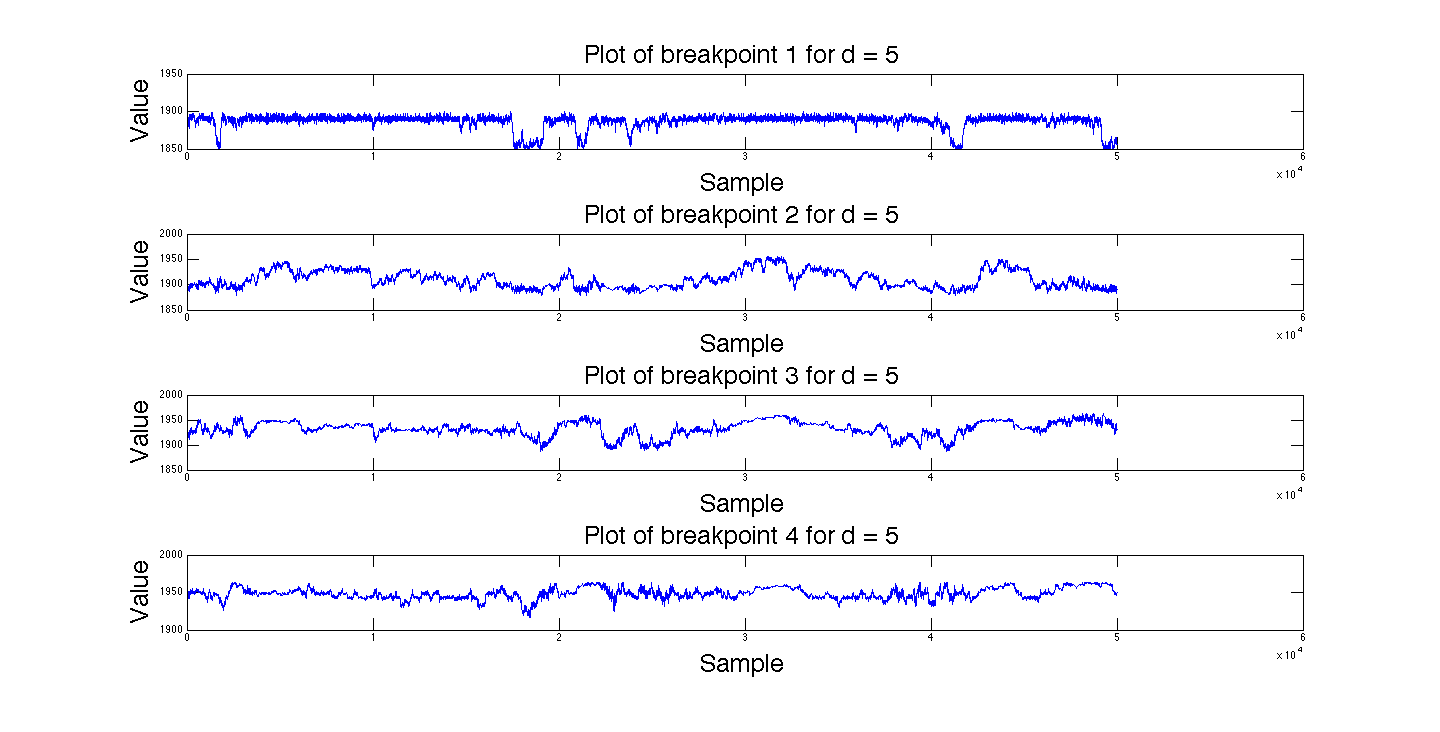
\includegraphics[scale=0.28]{./Figures/fixrho4.png}
  \label{fig:fixrho4}
\end{minipage}

  \caption[An Electron]{Figure of t-posterior for one and four breakpoints for a fixed constant $\rho=0.05$}
\end{figure}

One can deduce from the figures \ref{fig:fixrho1},\ref{fig:fixrho4} that the mixing is good for one breakpoint. However, we will have more correlated values when using $\rho=0.05$ for four breakpoints. Instead of using a constant $\rho$ we introduce a varing $\rho$ which is determined by the number of breakpoints used.

\begin{figure}[H]

  \centering
\begin{minipage}{1\textwidth}
    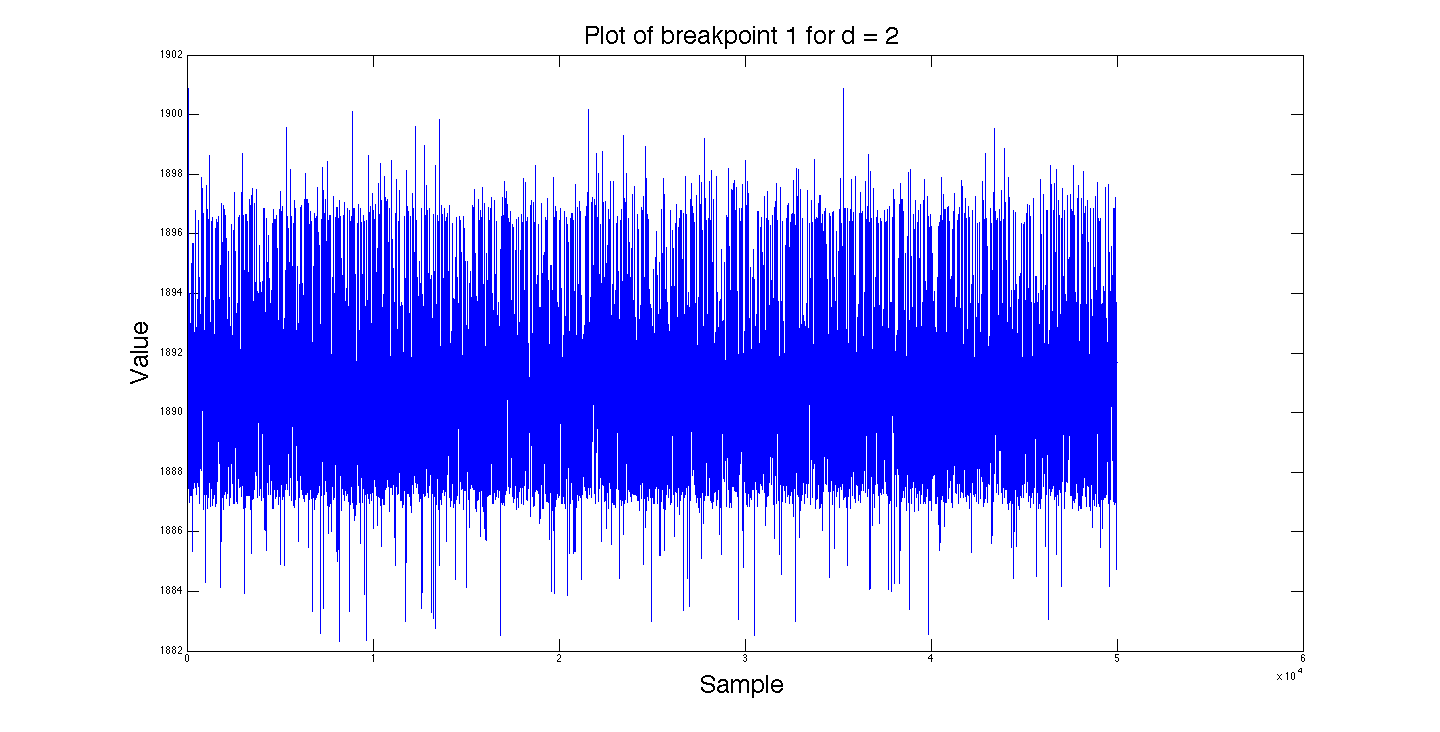
\includegraphics[scale=0.28]{./Figures/varrho1.png}
  \label{fig:varrho1}
\end{minipage}

\begin{minipage}{1\textwidth}
    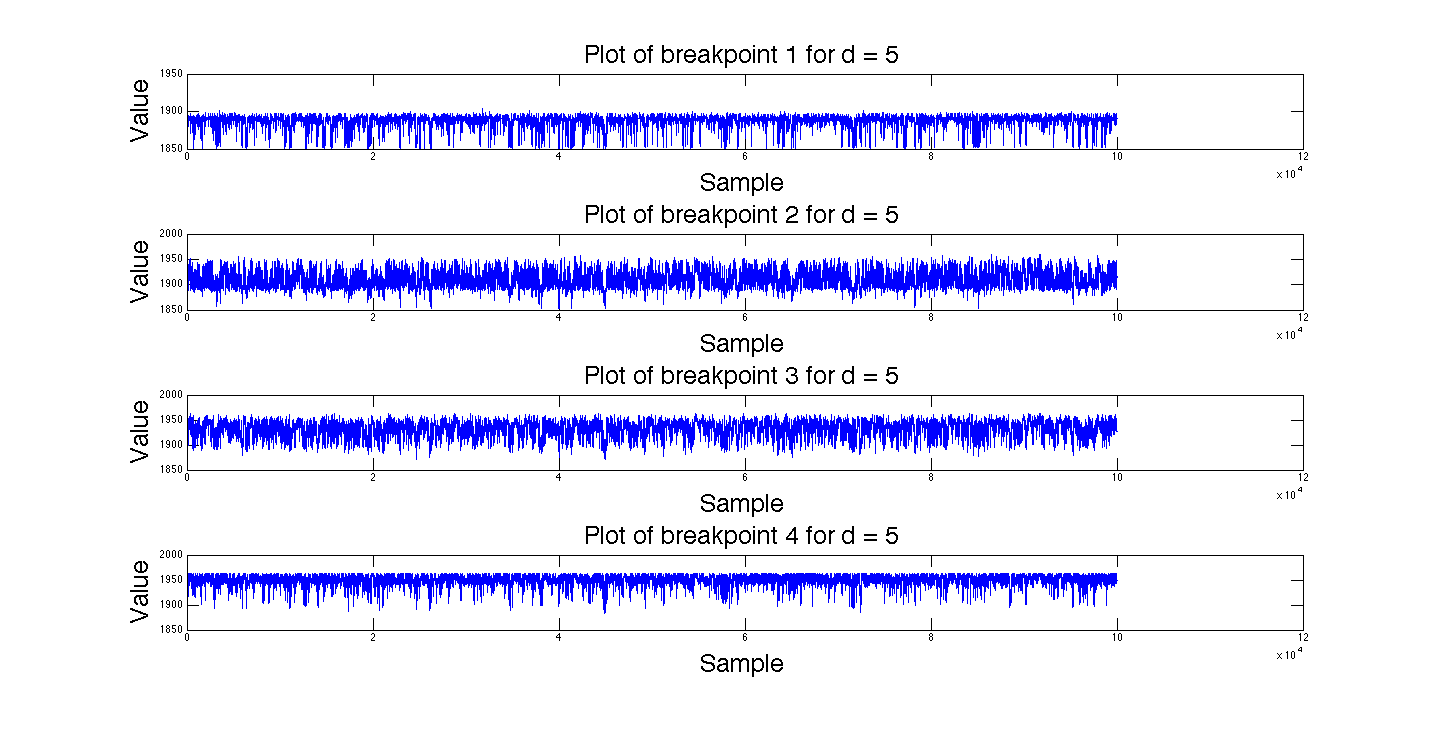
\includegraphics[scale=0.28]{./Figures/t4.png}
  \label{fig:varrho4}
\end{minipage}

  \caption[An Electron]{Figure of t-posterior for breakpoints$=1,4$ for a varing $\rho$}
\end{figure}

From the figures \ref{fig:varrho1},\ref{fig:varrho4} one can see that the mixing is more random and non-correlated compared with the fixed $\rho$. Indicating that our values should be better approximated using this relation.


\newpage
\section*{Parametric bootstrap method}
\subsection*{Introduction}

The problem consists of a dataset containing significant wave-heights recorded 14 times a month during several winter months in the north Atlantic. This is could for example be used to predict the probability of high waves in the north atlantic to warn oil platforms. One can estimate the extreme value of this dataset by assuming that the data has a \textit{Gumpel Distribution} with distribution function
\[ F(x; \mu, \beta)=\exp\left(-\exp\left(-\frac{x-\mu}{\beta}\right)\right), \quad x\in\mathbb{R}, \]
where $\mu\in\mathbb{R}$ and $\beta>0$. The paramaters of this distribution for an arbitrary dataset was estimated using the matlab function \texttt{est\_gumbel.m}. \\

During a 100 year interval, one can calculate a estimate of the likelihood of an 100--year return period event. It is a statistical measurement typically based on historic data denoting the average recurrence interval over an extended period of time. The analysis assumes that the probability does not vary in time and is independant of past events. \\

The expected 100-year return value of the data gives the largest expected wave-height during a 100-year period. The $T$:th return value is denoted by $F^{-1}(1-1/T;\mu,\beta)$. Since the data has been observed during 14 times a month and assuming we have three winter months during a year, $T$ is $T=3\cdot14\cdot100$. The investigated dataset is shown below in figure \ref{fig:waves}. \\

\begin{figure}[H]
\centering
	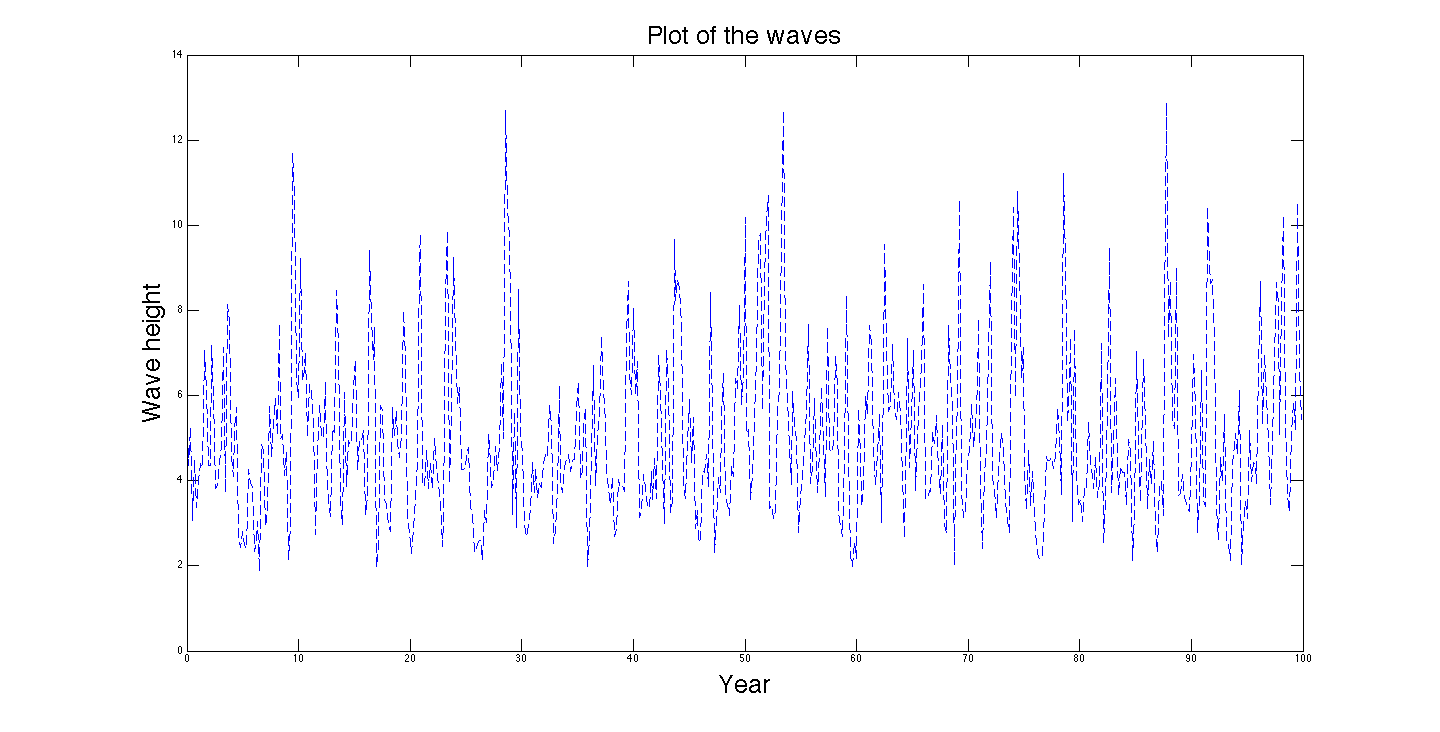
\includegraphics[scale=0.26]{./Figures/waves.png}
\caption{A figure, showing the data of the significant observed wave-heights}
\label{fig:waves}

\end{figure}

To perform a statistical test on the dataset, we use a parametric bootstrap approach. The bootstrap technique evaluates the uncertainty of an unknown distribution or data. The bootstrap replaces the unknown statistic by data-based approximations and analyzes the variation using MC simulation from the approximation. The approximations are done using a \textbf{empirical distribution} (ED) associated with the data and gives equal weights to each observed value. Below we will present a brief description of a general bootstrap method.

\begin{itemize}
\item{For a given statistic y, we replace $\mathbb{P}_0$ by $\hat{\mathbb{P}}_0$.}
\item{Approximation can be done by plugging $\hat{\mathbb{P}}_0$ into the quantity, i.e.
\[ \tau=\tau(\mathbb{P}_0)\approx \hat{\tau}=\tau(\hat{\mathbb{P}}_0) \].}
\item{Uncertainty of $t(y)$ is analyzed by looking at the variation of $\Delta(Y^*)=t(Y^*)-\hat{\tau}$ by drawing repeatedly $Y^*\sim \hat{\mathbb{P}_0}$.}
\end{itemize}

In our case, we have done a parametric bootstrap, where we assume that the data comes from a distribution $\mathbb{P}_0=\mathbb{P}_{\theta_0}\in\{\mathbb{P}_\theta;\theta \in \Theta\}$ belonging to some parametric family. Instead of using the ED, we find an estimate $\hat{\theta}=\hat{\theta}(y)$ of $\theta_0$ from the observations and
\begin{enumerate}
\item{generate new bootstrapped samples $Y_b^*,b\in \{1,2,\dots,B\}$, from $\hat{\mathbb{P}_0}=\mathbb{P}_{\hat{\theta}}$.}
\item{then we form bootstrap estimates $\hat{\theta}(Y_b^*)$ and errors $\Delta_b^*=\hat{\theta}(Y_b^*)-\hat{\theta},b\in\{1,2,\dots,B\}$}.
\end{enumerate}

For this assigment we approximated the data as being that of \textit{Gumpel distributed} data points. In the figure \ref{fig:waveshist} we have plotted the histogram of the atlantic wave-heights, indicating that the data has a a \textit{Gumpel} distribution.

\begin{figure}[H]
\centering
	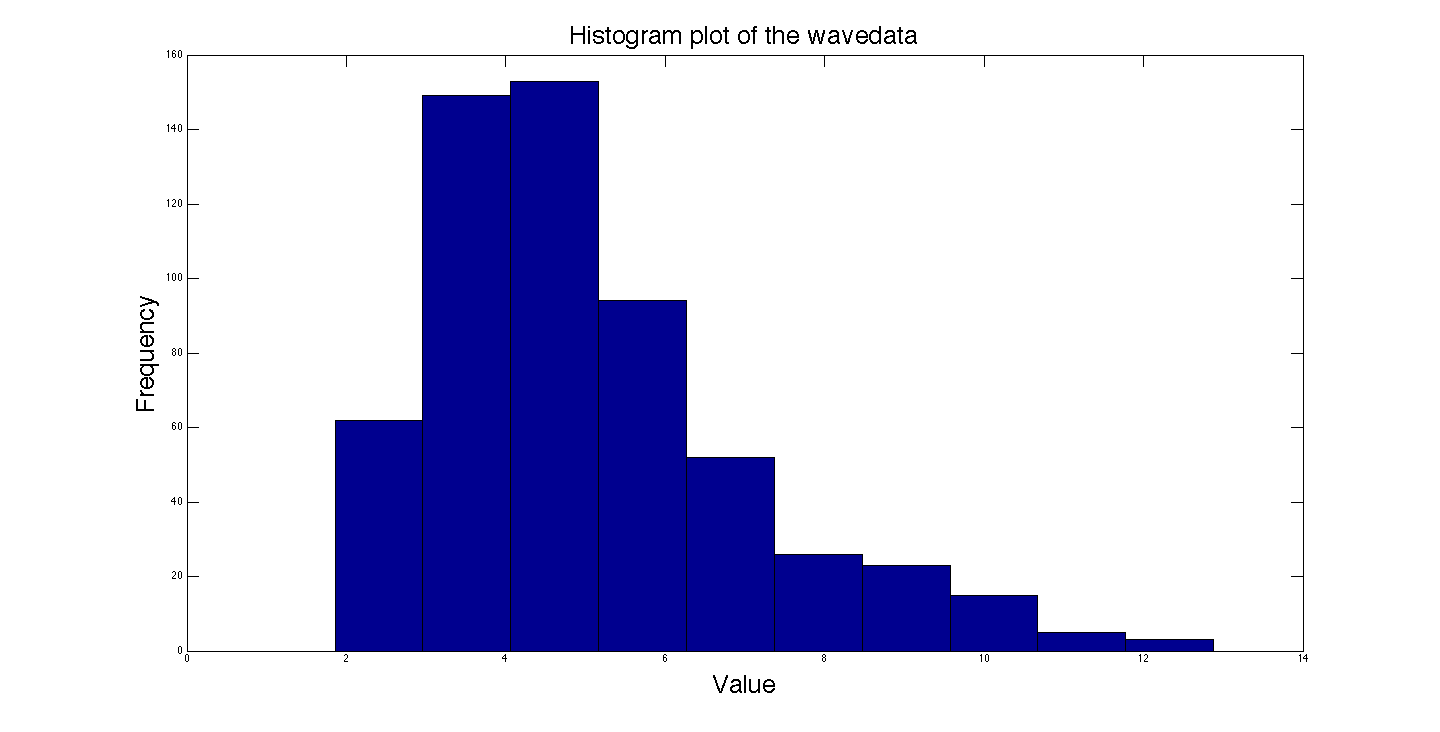
\includegraphics[scale=0.26]{./Figures/waveshist.png}
\caption{A figure, showing the data of the significant observed wave-heightsdata, in \texttt{atlantic.mat}}
\label{fig:waveshist}

\end{figure}


% \section*{Parametric Bootstrap for the 100-year Atlantic wave}

\subsection*{a)}
We will here find the inverse of the atlantic wave distribution, approximated as a \textit{Gumpel Distribution}. To begin finding an inverse we insert a new variable for the function and solve for x. This is done below

\[ F(x;\mu,\beta))=\exp\left(-\exp\left(-\frac{x-\mu}{\beta}\right)\right), x \in \mathbb{R} \]
Here we insert $u$ for the function
\begin{align*}
&u = \exp \left \{ -\exp\left(-\frac{x-\mu}{\beta}\right)\right\} \Rightarrow \ln(u)=-\exp\left(-\frac{x-\mu}{\beta}\right) \Rightarrow \\
& \ln\left\{\ln\left(\frac{1}{u}\right)\right\}=-\frac{x-\mu}{\beta} \Rightarrow \mu-\beta \ln \left \{\ln\left ( \frac{1}{u}\right ) \right \}=x.
\end{align*}


\subsection*{b)}
In this assignment we will provide a parametric bootstrapped 95\% confidence interval for the parameters. Since we have a dataset that we can evaluate parameters from, we need to determine the uncertainty of the estimators. To assess the uncertainty we analyze the distribution function $F_{\Delta}$ of the error $\Delta$ under $\mathbb{P}_0$. This uncertainty can be bounded by confidence intervals to assess the uncertainty we analyze the distribution function $F_{\Delta}$ of the error $\Delta$ under $\mathbb{P}_0$. \\

First of, we begin the bootstrap as described previously. We therefore estimate the parameters of the data by the function \texttt{est\_gumpel.m}. These estimates are the frequentistic approach using maximum likelihood. We then sample new data by generating random numbers and sampling using the inverse method of the relation derived in section \textbf{a)}. Thereafter we calculate the error of our estimates by the relation $\Delta_b^*(t)=\hat{t}_b^*-\hat{t}$. To get the confidence bounds for our estimates we used the relation \eqref{conf} derived in Jimmy Olssons lecture notes \cite{JO} 
\begin{equation} I_{\alpha}=\left(t(y) - F_\Delta^{-1}(F_\Delta^{-1}(1-\alpha/2),t(y)-F_\Delta^{-1}(\alpha/2)\right).
\label{conf}
 \end{equation}

However, we also need to check the bias of our estimate by the relation
\[ B_t=\mathbb{E}_0(t(Y)-\tau)=\mathbb{E}_0(\Delta(Y))=\int zf_\Delta (z) dz, \]
where $f_\Delta(z)=\frac{d}{dz}F_\Delta(z)$ denoting the density of $\Delta(Y)$. The calculated bias of the estimator for $\mu$ and $\beta$ respectively was computed as 
\[ B_t = \mathbb{E}_0(\Delta_b^*(t))=\left\{ \begin{array}{l}
-0.0009 \\ 0.0037
\end{array}\right. \]

The bias was then taken into consideration by making the bias-corrected estimate $t-B_t$. 

\begin{table}
\centering
\begin{tabular}{|c|c|c|}
\hline

 & L & U \\ \hline
%Estimates & 1.4858 & 4.1477 \\ \hline
$\beta$ & 1.3942 & 1.5821 \\ \hline
$\mu$ & 4.0220 & 4.2723 \\ \hline

\end{tabular}
\caption{Table showing the expected values and upper and lower bounds.}
\end{table}

In figure \ref{fig:estwaves} the histogram of the estimated dataset as well as the dataset is plotted.

\begin{figure}[H]
\centering
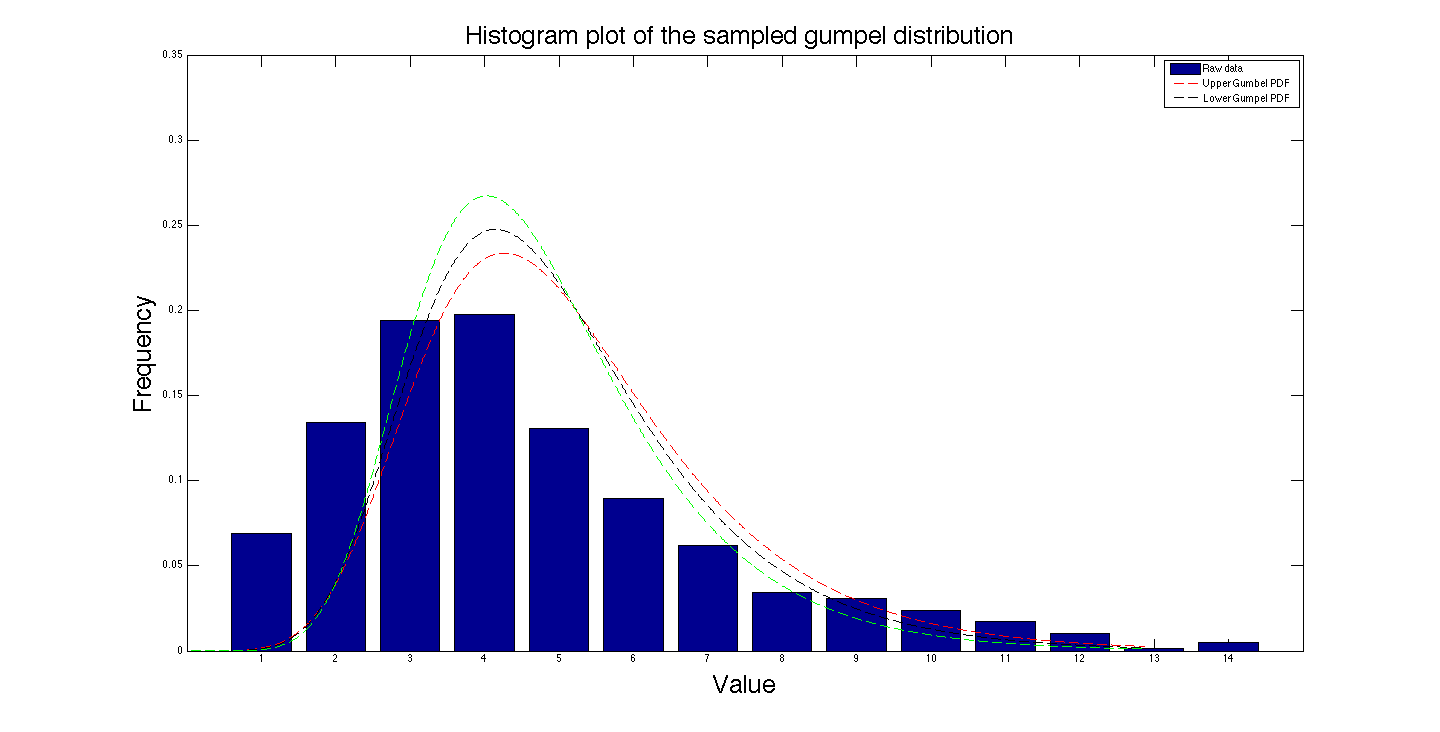
\includegraphics[scale=0.26]{./Figures/estwaves.png}

\label{fig:estwaves}
\caption{A histrogram of the estimated dataset, plotted over the real dataset.}
\end{figure} 

Here we can see the upper and lower cconfidence bound of the estimated wavesplotted with the raw data. One can observe that the gumpel approximation is indeed an approximation of the data.


\subsection*{c)}

For some datasets it is of interest to only calculate the upper/lower bound of the estimate. As for our case, one is not particularly interested in a significant wave-lengths lower bound, but rather the upper bound. Here we will provide a one-sided parametric bootstrapped 95\% confidence interval for the 100-year return value of the significant wave-height data provided. \\

If we want to get the return value of the 100-year return value, we use the relation derived in the introduction above. To recall it is denoted by
\[ F^{-1}(1-1/T;\mu,\beta), \quad T=3\cdot14\cdot100.\] \\

If we want to get the return value of the 100-year return value, we use the relation derived in the introduction above. To recall it is denoted by
\[ F^{-1}(1-1/T;\mu,\beta), \quad T=3\cdot14\cdot100.\]
To get the return value we therefore use the relation for the inverse again in assignment \textbf{a)} by inserting $u=1-1/T$ and our estimated $\mu$ and $\beta$. Giving the return value as
\[  \mu-\beta \ln \left \{\ln\left ( \frac{1}{u}\right ) \right \}=x,\quad x=16.5436\]

This is however, only the maximum-value using our estimates and if we use the same arguments as before. Meaning, we calculate the maximum-value using the relation, but we here use the upper bounds for our estimate. This returns the value $x=17.3984$. As a result, our one-sided 95\% confidence bound of the 100-year return value for the wave-height is 
\[ x_b=(16.5436,17.3984)\quad m \]


\begin{thebibliography}{99}
\bibitem{JO}
Olsson, J
\newblock
\emph{\href{http://www.math.kth.se/matstat/gru/sf2955/}{KTH course in Computer Intensive Methods}}

\end{thebibliography}


\end{document}
